\section{Experiment D}

\begin{minipage}{0.45\textwidth}
	\centering
	\begin{tabular}{lr}
	\toprule
	\textbf{Hyperparameter} & \textbf{Value} \\
	\midrule
	Buffer Size & \\
	Batch Size & \\
	Gamma ($\gamma$) & \\
	Tau ($\tau$) & \\
	Actor Learning Rate & \\
	Critic Learning Rate & \\
	Weight Decay & \\
	OU Noise Mu ($\mu$) & \\
	OU Noise Theta ($\theta$) & \\
	OU Noise Mu ($\sigma$) & \\
	\bottomrule
	\end{tabular}
\end{minipage}
\hspace{1cm}
\begin{minipage}{0.45\textwidth}
	\centering
	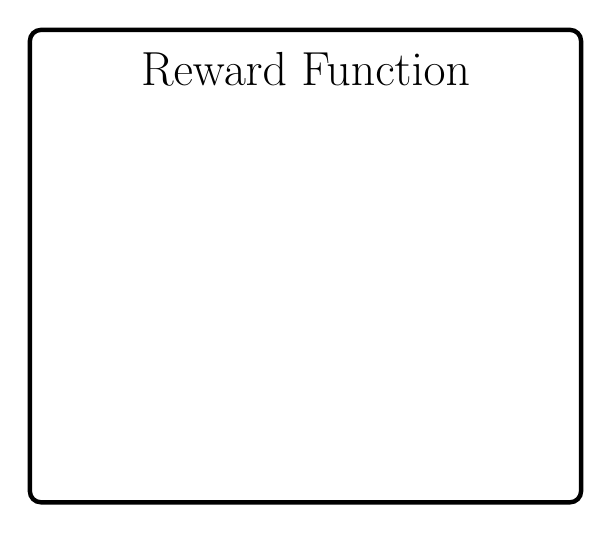
\begin{tikzpicture}
		\node (1) [draw, rectangle, minimum width=7cm, minimum height=6cm, rounded corners, ultra thick] {};
		\node at (0,2.5) {\LARGE Reward Function} ;
	\end{tikzpicture}
\end{minipage}

\begin{figure}[h]
	\begin{minipage}{0.45\textwidth}
		\centering
		% This file was created by tikzplotlib v0.9.1.
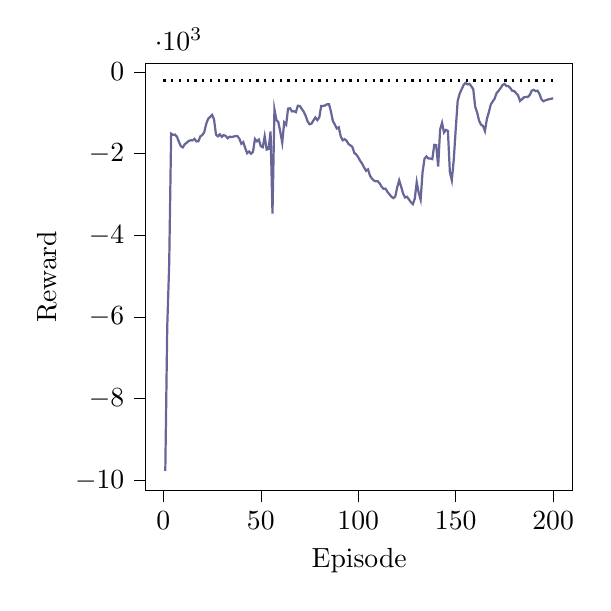
\begin{tikzpicture}

\definecolor{color0}{rgb}{0.12156862745098,0.466666666666667,0.705882352941177}

\begin{axis}[
compat=newest,
tick align=outside,
tick pos=left,
x grid style={white!69.0196078431373!black},
xmin=-8.95, xmax=209.95,
xtick style={color=black},
y grid style={white!69.0196078431373!black},
ymin=-10237.8868910548, ymax=203.619925054467,
ytick style={color=black},
scaled y ticks=true,
scaled y ticks=base 10:-3,
width=7cm,
height=7cm,
xlabel=Episode,
ylabel=Reward
]

\addplot[thick, black, dotted, domain=0:200] {-211.15};

\addplot [thick, blue!20!gray]
table {%
1 -9763.27294486799
2 -6233.80261025401
3 -4702.25607429109
4 -1512.21343297441
5 -1541.56062085325
6 -1535.22850284016
7 -1588.96606184897
8 -1715.23669898396
9 -1820.31231753912
10 -1847.66786072394
11 -1769.92450118555
12 -1734.64730574001
13 -1691.78106317152
14 -1674.45493906621
15 -1676.90591264538
16 -1640.75523295968
17 -1703.4048995174
18 -1697.83044713235
19 -1576.88921890067
20 -1546.5715732237
21 -1474.09512876949
22 -1271.65422689584
23 -1150.29854596291
24 -1102.56488295819
25 -1052.63460403206
26 -1160.0570975787
27 -1531.80428427574
28 -1577.96536228338
29 -1528.46964853933
30 -1588.81698896337
31 -1545.80968137986
32 -1568.85552000374
33 -1624.20152414619
34 -1586.50471460737
35 -1592.55986202214
36 -1584.94638344089
37 -1569.33361174512
38 -1573.1892994717
39 -1633.50494911412
40 -1759.32305467967
41 -1719.13862961987
42 -1862.97480239258
43 -1990.60310329712
44 -1948.10280201805
45 -2003.32412321478
46 -1956.29505058938
47 -1643.40355154487
48 -1699.32053231105
49 -1655.76163636967
50 -1820.85636906421
51 -1844.26667355161
52 -1574.87178814199
53 -1901.6723073915
54 -1886.04289052694
55 -1458.04140202327
56 -3469.32441220565
57 -917.195658586486
58 -1176.59257034398
59 -1230.33078309159
60 -1466.59633331869
61 -1732.22292637077
62 -1236.42594346941
63 -1293.97326214233
64 -899.857651460993
65 -890.845587246339
66 -968.24154739275
67 -963.199443956724
68 -986.677853906075
69 -828.526039545684
70 -834.720257437712
71 -902.709529703026
72 -972.62043534064
73 -1074.17044214855
74 -1209.87366623514
75 -1283.68681382054
76 -1267.54188154102
77 -1187.55869135607
78 -1114.1130550254
79 -1179.99960886007
80 -1115.99943619309
81 -832.657288986692
82 -832.72759717624
83 -822.279758669418
84 -793.164073797469
85 -791.044522604899
86 -972.019086460731
87 -1206.24867561322
88 -1290.02850233563
89 -1384.86591544101
90 -1357.00442247666
91 -1575.38270406248
92 -1674.08821396743
93 -1647.60414166174
94 -1684.15617335132
95 -1765.71695848599
96 -1797.33452011673
97 -1838.75461128161
98 -1985.76014825974
99 -2021.98376684527
100 -2092.02233018191
101 -2178.15994993705
102 -2247.02313410243
103 -2340.33340175948
104 -2420.7367742868
105 -2385.67777225085
106 -2538.2164437452
107 -2609.81411422946
108 -2659.40383450713
109 -2678.50832692135
110 -2676.82744132636
111 -2730.33624432342
112 -2812.33229768694
113 -2861.50305884707
114 -2857.37029123113
115 -2938.78510578548
116 -2994.46766053733
117 -3054.18167696401
118 -3089.68136986634
119 -3050.40051346782
120 -2823.26624003158
121 -2653.39029885552
122 -2806.59146922999
123 -2978.05949681073
124 -3075.60138846972
125 -3056.50890159285
126 -3119.86383000792
127 -3190.77697519937
128 -3237.45041767532
129 -3103.94340263226
130 -2698.75288944802
131 -2956.79624472601
132 -3124.84788885606
133 -2453.99592562811
134 -2125.61227356192
135 -2067.71562137431
136 -2118.05416804509
137 -2120.76157358531
138 -2134.78314728543
139 -1786.15300160098
140 -1793.00208055793
141 -2319.18931540986
142 -1413.05062097296
143 -1245.7107253682
144 -1484.37154592392
145 -1420.74714969691
146 -1446.61374769009
147 -2448.65824563979
148 -2652.9204998935
149 -2151.41685205676
150 -1409.62535384097
151 -715.425293566961
152 -537.233050162036
153 -429.756832729694
154 -325.6823376965
155 -270.994021132317
156 -306.189756950749
157 -292.000625606546
158 -350.489728088838
159 -423.619606641182
160 -855.467889009458
161 -994.472702683325
162 -1195.21463389004
163 -1292.79692031924
164 -1320.56851018644
165 -1448.16350042877
166 -1152.54457203662
167 -987.150718369486
168 -798.086323275897
169 -722.281160318246
170 -651.843048097534
171 -517.090294083444
172 -462.655401350926
173 -399.143888792889
174 -324.173287068825
175 -295.147502477148
176 -344.83352622425
177 -349.652649290451
178 -394.784026316548
179 -462.079584436464
180 -468.014634507583
181 -522.962154721305
182 -573.619728760075
183 -711.92181205646
184 -671.105200941416
185 -622.486488273209
186 -613.495902939192
187 -614.457292613144
188 -566.095980332205
189 -462.064404335876
190 -440.344339674872
191 -470.810273558386
192 -460.606507255502
193 -542.73700519533
194 -671.942780564072
195 -720.097164404344
196 -696.536841144416
197 -680.892791035771
198 -667.588830250088
199 -657.904337807085
200 -646.907259376791
};
\end{axis}

\end{tikzpicture}

		\caption{text}
		\label{fig:5401_raw_reward}
	\end{minipage}
	\hspace{0.75cm}
	\begin{minipage}{0.45\textwidth}
		\centering
		% This file was created by tikzplotlib v0.9.1.
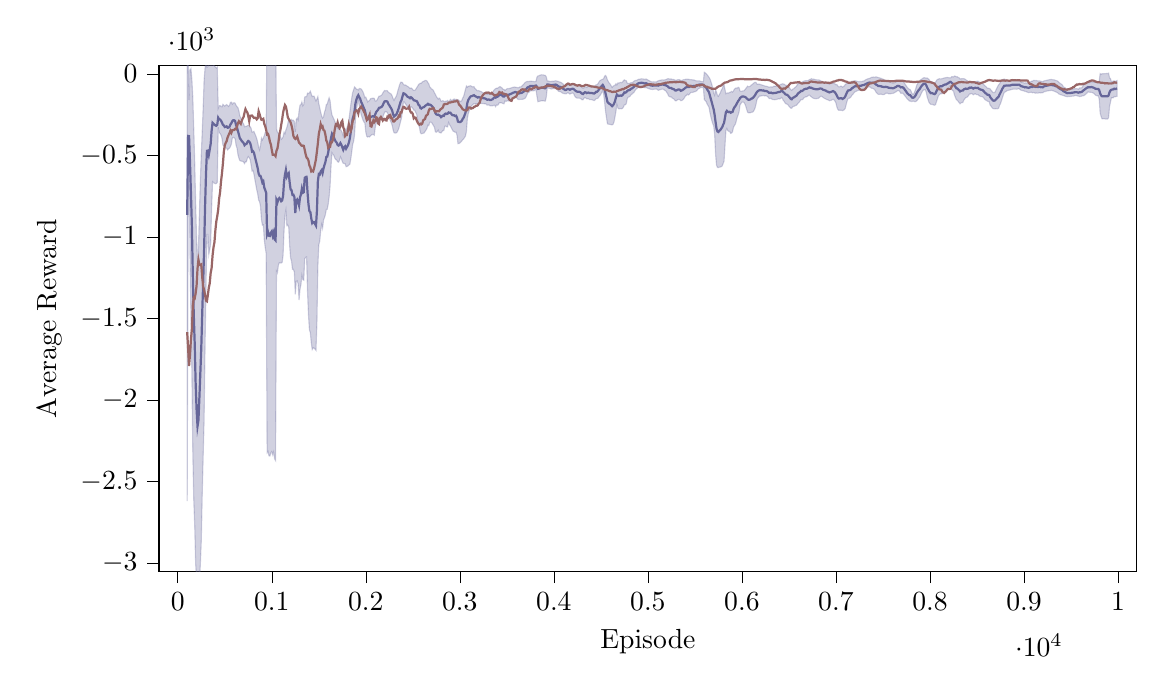
\begin{tikzpicture}

\definecolor{color0}{rgb}{1,0.498039215686275,0.0549019607843137}
\definecolor{color1}{rgb}{0.12156862745098,0.466666666666667,0.705882352941177}

\begin{axis}[
compat=newest,
tick align=outside,
tick pos=left,
x grid style={white!69.0196078431373!black},
xmin=-200.00, xmax=10200.00,
xtick style={color=black},
y grid style={white!69.0196078431373!black},
ymin=-3050.00, ymax=50.00,
ytick style={color=black},
scaled y ticks=true,
scaled y ticks=base 10:-3,
width=14cm,
height=8cm,
xlabel=Episode,
ylabel=Average Reward,
%y label style={at={(-0.2,0.5)}}
]

\path [draw=blue!20!gray, fill=blue!20!gray, opacity=0.3]
(axis cs:100,-2619.66152671753)
--(axis cs:100,892.158016068593)
--(axis cs:110,143.417432403521)
--(axis cs:120,-159.868663228158)
--(axis cs:130,24.7893742445649)
--(axis cs:140,33.333554046847)
--(axis cs:150,-33.2642814496542)
--(axis cs:160,-143.657189695485)
--(axis cs:170,-336.157031576302)
--(axis cs:180,-537.612239198292)
--(axis cs:190,-786.829676239442)
--(axis cs:200,-1012.18569074914)
--(axis cs:210,-1164.84716706992)
--(axis cs:220,-1066.52010638052)
--(axis cs:230,-853.336857007459)
--(axis cs:240,-657.089152134831)
--(axis cs:250,-493.044624742404)
--(axis cs:260,-354.251041991786)
--(axis cs:270,-207.968814158809)
--(axis cs:280,-36.041658426059)
--(axis cs:290,35.3951059587054)
--(axis cs:300,81.0433027675488)
--(axis cs:310,41.7851044334526)
--(axis cs:320,45.822575547255)
--(axis cs:330,115.543280671045)
--(axis cs:340,151.042035697885)
--(axis cs:350,184.924506173131)
--(axis cs:360,127.169113813713)
--(axis cs:370,63.8890578763668)
--(axis cs:380,57.4067109192207)
--(axis cs:390,50.6463358980554)
--(axis cs:400,42.7116077693309)
--(axis cs:410,37.0946392685346)
--(axis cs:420,42.2397167739448)
--(axis cs:430,-209.545595485802)
--(axis cs:440,-194.362869205383)
--(axis cs:450,-193.008142741514)
--(axis cs:460,-198.105684239587)
--(axis cs:470,-200.814825797196)
--(axis cs:480,-185.785044351546)
--(axis cs:490,-190.887600001776)
--(axis cs:500,-196.213660413729)
--(axis cs:510,-191.178715658053)
--(axis cs:520,-186.800473308824)
--(axis cs:530,-192.440170229498)
--(axis cs:540,-198.721705253067)
--(axis cs:550,-192.046332400587)
--(axis cs:560,-173.480616988425)
--(axis cs:570,-172.034525270181)
--(axis cs:580,-184.966025574163)
--(axis cs:590,-177.48207209218)
--(axis cs:600,-175.850621769989)
--(axis cs:610,-178.576897496839)
--(axis cs:620,-191.535040945691)
--(axis cs:630,-200.482812824836)
--(axis cs:640,-206.521766527551)
--(axis cs:650,-225.528927744388)
--(axis cs:660,-256.720712729266)
--(axis cs:670,-268.20219468699)
--(axis cs:680,-285.46056867786)
--(axis cs:690,-297.532782383731)
--(axis cs:700,-305.480136443816)
--(axis cs:710,-323.458764231164)
--(axis cs:720,-321.484351175558)
--(axis cs:730,-320.938622254352)
--(axis cs:740,-317.104020625761)
--(axis cs:750,-314.723629157764)
--(axis cs:760,-314.192825855059)
--(axis cs:770,-322.386282087952)
--(axis cs:780,-332.410424032999)
--(axis cs:790,-356.368661452699)
--(axis cs:800,-354.867942642454)
--(axis cs:810,-351.390476954994)
--(axis cs:820,-365.760643221369)
--(axis cs:830,-379.652937977043)
--(axis cs:840,-395.323525431777)
--(axis cs:850,-418.603542566595)
--(axis cs:860,-446.927768973098)
--(axis cs:870,-464.882437733692)
--(axis cs:880,-437.838875465213)
--(axis cs:890,-392.698877006504)
--(axis cs:900,-404.164732240528)
--(axis cs:910,-391.577765095429)
--(axis cs:920,-378.100482784936)
--(axis cs:930,-358.457665643661)
--(axis cs:940,-355.944545277711)
--(axis cs:950,354.704127095817)
--(axis cs:960,377.155933963715)
--(axis cs:970,357.573138550829)
--(axis cs:980,356.279106701561)
--(axis cs:990,375.005344102528)
--(axis cs:1000,385.229679860142)
--(axis cs:1010,352.65646205148)
--(axis cs:1020,373.95297769975)
--(axis cs:1030,333.286038000532)
--(axis cs:1040,329.97582236349)
--(axis cs:1050,-337.632534220744)
--(axis cs:1060,-356.644667650016)
--(axis cs:1070,-363.04632399173)
--(axis cs:1080,-363.35000298447)
--(axis cs:1090,-377.400761837185)
--(axis cs:1100,-400.938779563579)
--(axis cs:1110,-394.832134739012)
--(axis cs:1120,-385.220213337792)
--(axis cs:1130,-356.968423128672)
--(axis cs:1140,-365.745000055487)
--(axis cs:1150,-342.616415084686)
--(axis cs:1160,-327.506267741536)
--(axis cs:1170,-304.373936611007)
--(axis cs:1180,-277.579701841541)
--(axis cs:1190,-276.947049770174)
--(axis cs:1200,-287.210812936337)
--(axis cs:1210,-278.891980329164)
--(axis cs:1220,-285.335720867453)
--(axis cs:1230,-283.289014955501)
--(axis cs:1240,-291.900022041836)
--(axis cs:1250,-354.146009756239)
--(axis cs:1260,-278.642151955696)
--(axis cs:1270,-269.889973502971)
--(axis cs:1280,-281.324404314355)
--(axis cs:1290,-226.306696651361)
--(axis cs:1300,-191.134363254425)
--(axis cs:1310,-186.637121654118)
--(axis cs:1320,-171.204821332552)
--(axis cs:1330,-194.929089656005)
--(axis cs:1340,-185.292033062251)
--(axis cs:1350,-140.958121912397)
--(axis cs:1360,-138.14485614994)
--(axis cs:1370,-138.743465901711)
--(axis cs:1380,-117.037579418467)
--(axis cs:1390,-119.348802660256)
--(axis cs:1400,-114.779674183922)
--(axis cs:1410,-105.005412808382)
--(axis cs:1420,-121.939709443431)
--(axis cs:1430,-138.383617163136)
--(axis cs:1440,-135.318186096051)
--(axis cs:1450,-135.192465435235)
--(axis cs:1460,-151.909694150803)
--(axis cs:1470,-165.272413923004)
--(axis cs:1480,-153.072874370195)
--(axis cs:1490,-138.195722760184)
--(axis cs:1500,-180.328448711017)
--(axis cs:1510,-207.412123580352)
--(axis cs:1520,-233.874051807909)
--(axis cs:1530,-256.907380952397)
--(axis cs:1540,-269.644580906817)
--(axis cs:1550,-262.498722309743)
--(axis cs:1560,-234.908759080975)
--(axis cs:1570,-217.97332682647)
--(axis cs:1580,-187.025050849085)
--(axis cs:1590,-183.363956225357)
--(axis cs:1600,-162.614885702122)
--(axis cs:1610,-145.468010116827)
--(axis cs:1620,-162.338535946054)
--(axis cs:1630,-217.853338074827)
--(axis cs:1640,-250.497648983556)
--(axis cs:1650,-263.476968025274)
--(axis cs:1660,-275.836245914643)
--(axis cs:1670,-289.718697122411)
--(axis cs:1680,-304.535968552059)
--(axis cs:1690,-312.799029659845)
--(axis cs:1700,-331.776137049109)
--(axis cs:1710,-336.894900148893)
--(axis cs:1720,-338.83332699433)
--(axis cs:1730,-338.946828676747)
--(axis cs:1740,-347.749577246733)
--(axis cs:1750,-360.882730361436)
--(axis cs:1760,-381.353448880537)
--(axis cs:1770,-350.651860665683)
--(axis cs:1780,-336.66532092883)
--(axis cs:1790,-347.046930145209)
--(axis cs:1800,-328.109570835285)
--(axis cs:1810,-309.734915461839)
--(axis cs:1820,-281.631398869983)
--(axis cs:1830,-234.996290762972)
--(axis cs:1840,-188.532285077493)
--(axis cs:1850,-147.786607715002)
--(axis cs:1860,-113.981250671092)
--(axis cs:1870,-96.8355931440155)
--(axis cs:1880,-78.4892552807005)
--(axis cs:1890,-84.5225736281999)
--(axis cs:1900,-92.9212127169246)
--(axis cs:1910,-93.8106670422002)
--(axis cs:1920,-97.7369601814344)
--(axis cs:1930,-88.6032148203439)
--(axis cs:1940,-89.1270246771362)
--(axis cs:1950,-91.2702624421496)
--(axis cs:1960,-99.6431950986728)
--(axis cs:1970,-109.747016591405)
--(axis cs:1980,-124.975840452151)
--(axis cs:1990,-145.608612026297)
--(axis cs:2000,-141.708202372283)
--(axis cs:2010,-155.625330495793)
--(axis cs:2020,-170.640688805204)
--(axis cs:2030,-165.852803220698)
--(axis cs:2040,-161.148193018152)
--(axis cs:2050,-150.503155611278)
--(axis cs:2060,-150.131855068133)
--(axis cs:2070,-147.983268367726)
--(axis cs:2080,-147.383799186714)
--(axis cs:2090,-149.13059920936)
--(axis cs:2100,-165.423265004765)
--(axis cs:2110,-165.20022779846)
--(axis cs:2120,-159.228280784265)
--(axis cs:2130,-146.457132736993)
--(axis cs:2140,-135.778297887046)
--(axis cs:2150,-134.909933574662)
--(axis cs:2160,-132.010962950096)
--(axis cs:2170,-127.700741424813)
--(axis cs:2180,-116.736581312811)
--(axis cs:2190,-107.620728293087)
--(axis cs:2200,-100.471191549448)
--(axis cs:2210,-102.783781995596)
--(axis cs:2220,-100.967367083082)
--(axis cs:2230,-102.509222013596)
--(axis cs:2240,-112.121538464992)
--(axis cs:2250,-115.398812457873)
--(axis cs:2260,-119.19390610617)
--(axis cs:2270,-122.930846303379)
--(axis cs:2280,-133.49802279579)
--(axis cs:2290,-150.086552170513)
--(axis cs:2300,-161.458268487749)
--(axis cs:2310,-149.423435140194)
--(axis cs:2320,-139.734050971882)
--(axis cs:2330,-126.865946561438)
--(axis cs:2340,-103.559005234384)
--(axis cs:2350,-84.4920143081571)
--(axis cs:2360,-64.3428803505339)
--(axis cs:2370,-50.4734286590739)
--(axis cs:2380,-49.1996519060509)
--(axis cs:2390,-51.8640690255408)
--(axis cs:2400,-64.0959657896819)
--(axis cs:2410,-67.5282562512949)
--(axis cs:2420,-67.0718206516418)
--(axis cs:2430,-69.9507001797919)
--(axis cs:2440,-74.1745728595707)
--(axis cs:2450,-77.6014481677419)
--(axis cs:2460,-81.9360767910912)
--(axis cs:2470,-87.641853162809)
--(axis cs:2480,-84.9772296201055)
--(axis cs:2490,-88.3706143095472)
--(axis cs:2500,-96.7296319242037)
--(axis cs:2510,-99.8121272350313)
--(axis cs:2520,-100.388085672837)
--(axis cs:2530,-94.1740456391669)
--(axis cs:2540,-84.7995843391016)
--(axis cs:2550,-75.8353810092304)
--(axis cs:2560,-65.0986207079413)
--(axis cs:2570,-59.8944741350584)
--(axis cs:2580,-55.9146129888595)
--(axis cs:2590,-57.2847306551467)
--(axis cs:2600,-48.4551184122773)
--(axis cs:2610,-45.0113932792786)
--(axis cs:2620,-43.4957502719891)
--(axis cs:2630,-38.8901868334178)
--(axis cs:2640,-39.1642403409722)
--(axis cs:2650,-42.0087048291381)
--(axis cs:2660,-52.5897105094553)
--(axis cs:2670,-60.2929383475316)
--(axis cs:2680,-78.6148839985552)
--(axis cs:2690,-84.461534571542)
--(axis cs:2700,-91.8122723158397)
--(axis cs:2710,-94.1860239847056)
--(axis cs:2720,-101.501891234605)
--(axis cs:2730,-114.812837940954)
--(axis cs:2740,-124.369677960658)
--(axis cs:2750,-137.29490540979)
--(axis cs:2760,-146.195082160443)
--(axis cs:2770,-153.628377344503)
--(axis cs:2780,-147.137775262949)
--(axis cs:2790,-152.124400018845)
--(axis cs:2800,-167.35682964636)
--(axis cs:2810,-165.451099023495)
--(axis cs:2820,-163.277932040873)
--(axis cs:2830,-166.566581198333)
--(axis cs:2840,-170.622952909282)
--(axis cs:2850,-165.668799190569)
--(axis cs:2860,-166.495778385167)
--(axis cs:2870,-161.970961089955)
--(axis cs:2880,-173.617454856077)
--(axis cs:2890,-165.232779181777)
--(axis cs:2900,-155.441871003052)
--(axis cs:2910,-160.889034248909)
--(axis cs:2920,-161.507048387956)
--(axis cs:2930,-155.927613443131)
--(axis cs:2940,-152.735091343907)
--(axis cs:2950,-157.701953590104)
--(axis cs:2960,-154.848216422665)
--(axis cs:2970,-159.181896383476)
--(axis cs:2980,-156.386560719864)
--(axis cs:2990,-160.796982480326)
--(axis cs:3000,-166.909379369568)
--(axis cs:3010,-167.05340426563)
--(axis cs:3020,-163.252177292394)
--(axis cs:3030,-147.426476302125)
--(axis cs:3040,-137.708438371378)
--(axis cs:3050,-116.404623875368)
--(axis cs:3060,-93.6429361810282)
--(axis cs:3070,-73.3673712699593)
--(axis cs:3080,-80.2794852020606)
--(axis cs:3090,-74.2531811585503)
--(axis cs:3100,-74.2156595579071)
--(axis cs:3110,-71.4539817854838)
--(axis cs:3120,-72.8230726914501)
--(axis cs:3130,-78.0250521913816)
--(axis cs:3140,-78.1595264375167)
--(axis cs:3150,-77.0021904112291)
--(axis cs:3160,-87.8821541751977)
--(axis cs:3170,-92.2845438607121)
--(axis cs:3180,-99.7746076712901)
--(axis cs:3190,-103.102400203989)
--(axis cs:3200,-101.176247151843)
--(axis cs:3210,-104.155500423861)
--(axis cs:3220,-106.403336727915)
--(axis cs:3230,-107.906005634431)
--(axis cs:3240,-113.026638069747)
--(axis cs:3250,-115.580668994561)
--(axis cs:3260,-115.147379526974)
--(axis cs:3270,-118.540202515621)
--(axis cs:3280,-121.400791646834)
--(axis cs:3290,-124.194672272525)
--(axis cs:3300,-123.187005786357)
--(axis cs:3310,-122.9819163256)
--(axis cs:3320,-125.299932460293)
--(axis cs:3330,-123.98184555356)
--(axis cs:3340,-116.7717628811)
--(axis cs:3350,-113.627941932947)
--(axis cs:3360,-100.200355138066)
--(axis cs:3370,-95.2463889407936)
--(axis cs:3380,-89.3100162073628)
--(axis cs:3390,-86.7775474618867)
--(axis cs:3400,-86.8484859248177)
--(axis cs:3410,-83.2455865299779)
--(axis cs:3420,-78.0878495979513)
--(axis cs:3430,-77.8068963634078)
--(axis cs:3440,-81.4772185317906)
--(axis cs:3450,-85.9351943003148)
--(axis cs:3460,-93.5069590216729)
--(axis cs:3470,-94.4264826542861)
--(axis cs:3480,-100.519511918809)
--(axis cs:3490,-95.5162812809998)
--(axis cs:3500,-90.4052734406122)
--(axis cs:3510,-88.587094373984)
--(axis cs:3520,-89.3474234319558)
--(axis cs:3530,-87.8569071901336)
--(axis cs:3540,-86.3239327074194)
--(axis cs:3550,-84.2358311499127)
--(axis cs:3560,-82.4226215876358)
--(axis cs:3570,-80.3549168799665)
--(axis cs:3580,-79.5118663245157)
--(axis cs:3590,-80.4133133547494)
--(axis cs:3600,-81.4487325847821)
--(axis cs:3610,-82.5983691618592)
--(axis cs:3620,-84.2122700320515)
--(axis cs:3630,-81.5392335991048)
--(axis cs:3640,-78.3751254888106)
--(axis cs:3650,-78.6334377186492)
--(axis cs:3660,-73.8450492860034)
--(axis cs:3670,-67.9809084883458)
--(axis cs:3680,-61.7678279081983)
--(axis cs:3690,-54.3889133777194)
--(axis cs:3700,-50.1206397339623)
--(axis cs:3710,-45.9550479716405)
--(axis cs:3720,-45.4300291792869)
--(axis cs:3730,-45.9616455763772)
--(axis cs:3740,-44.7144308287315)
--(axis cs:3750,-43.0975635625884)
--(axis cs:3760,-43.5293190664401)
--(axis cs:3770,-44.6900419989531)
--(axis cs:3780,-44.89803284693)
--(axis cs:3790,-46.8381400805137)
--(axis cs:3800,-45.6822856681009)
--(axis cs:3810,-44.9658600548566)
--(axis cs:3820,-19.1651497916726)
--(axis cs:3830,-11.4719143196953)
--(axis cs:3840,-10.6057006305912)
--(axis cs:3850,-7.51070714897452)
--(axis cs:3860,-5.52487209629902)
--(axis cs:3870,-4.41828620717594)
--(axis cs:3880,-5.02941140121533)
--(axis cs:3890,-5.45480272399421)
--(axis cs:3900,-7.59492235334048)
--(axis cs:3910,-8.01886658241229)
--(axis cs:3920,-18.4965017964236)
--(axis cs:3930,-42.9273592188371)
--(axis cs:3940,-42.4073774736956)
--(axis cs:3950,-44.0990213344708)
--(axis cs:3960,-44.7129088205628)
--(axis cs:3970,-45.0743820205543)
--(axis cs:3980,-44.0881999424697)
--(axis cs:3990,-44.4247869416037)
--(axis cs:4000,-43.8229966051183)
--(axis cs:4010,-42.0031254910825)
--(axis cs:4020,-41.0424576038621)
--(axis cs:4030,-42.9133047166713)
--(axis cs:4040,-43.1250893714026)
--(axis cs:4050,-46.1859241120426)
--(axis cs:4060,-48.3241077899119)
--(axis cs:4070,-49.7089853308752)
--(axis cs:4080,-52.7922294868954)
--(axis cs:4090,-56.9609329917177)
--(axis cs:4100,-62.3781405531513)
--(axis cs:4110,-68.331771661124)
--(axis cs:4120,-73.3099504140499)
--(axis cs:4130,-72.1895595499959)
--(axis cs:4140,-69.4700913217398)
--(axis cs:4150,-67.6123903133501)
--(axis cs:4160,-67.6537605968853)
--(axis cs:4170,-69.3880383414908)
--(axis cs:4180,-67.3317179679354)
--(axis cs:4190,-64.4702250693561)
--(axis cs:4200,-63.8818779022713)
--(axis cs:4210,-63.8993535441474)
--(axis cs:4220,-60.8605231070749)
--(axis cs:4230,-62.9041997362254)
--(axis cs:4240,-66.6320704221351)
--(axis cs:4250,-68.7019440976412)
--(axis cs:4260,-69.5356405435738)
--(axis cs:4270,-69.6810009378869)
--(axis cs:4280,-73.0557726553427)
--(axis cs:4290,-78.104104868626)
--(axis cs:4300,-83.3054940015446)
--(axis cs:4310,-86.9475873951711)
--(axis cs:4320,-84.8676840635295)
--(axis cs:4330,-79.2280885200349)
--(axis cs:4340,-78.4715975581839)
--(axis cs:4350,-81.6311122113981)
--(axis cs:4360,-77.1454749488615)
--(axis cs:4370,-75.0389334875152)
--(axis cs:4380,-76.3929337902294)
--(axis cs:4390,-75.4149025787929)
--(axis cs:4400,-75.253746775539)
--(axis cs:4410,-75.5271431086851)
--(axis cs:4420,-75.6005406174395)
--(axis cs:4430,-76.7746192577376)
--(axis cs:4440,-71.8942443138972)
--(axis cs:4450,-65.7123484264105)
--(axis cs:4460,-65.6288169259693)
--(axis cs:4470,-58.6427618897622)
--(axis cs:4480,-48.601894446837)
--(axis cs:4490,-40.4997144313107)
--(axis cs:4500,-36.8458557783056)
--(axis cs:4510,-33.7671567974635)
--(axis cs:4520,-32.4178018468791)
--(axis cs:4530,-27.090705612378)
--(axis cs:4540,-12.5787890667753)
--(axis cs:4550,-8.5700821973135)
--(axis cs:4560,-18.1523101010335)
--(axis cs:4570,-36.2501234284046)
--(axis cs:4580,-46.5766663271783)
--(axis cs:4590,-56.3896033398147)
--(axis cs:4600,-62.1406727209712)
--(axis cs:4610,-72.6874406563354)
--(axis cs:4620,-82.2597760693144)
--(axis cs:4630,-74.0134880118854)
--(axis cs:4640,-70.9834999877238)
--(axis cs:4650,-69.0672146635129)
--(axis cs:4660,-59.2603760962403)
--(axis cs:4670,-66.3750311668248)
--(axis cs:4680,-54.3827324260913)
--(axis cs:4690,-54.9946834109574)
--(axis cs:4700,-53.0620435347882)
--(axis cs:4710,-50.586216915131)
--(axis cs:4720,-52.9308519966821)
--(axis cs:4730,-47.5277281797751)
--(axis cs:4740,-41.2258338228806)
--(axis cs:4750,-35.6758637478907)
--(axis cs:4760,-39.5952498695448)
--(axis cs:4770,-40.3121018145199)
--(axis cs:4780,-55.2612353006627)
--(axis cs:4790,-57.7952519365008)
--(axis cs:4800,-57.8553665542449)
--(axis cs:4810,-56.2749669220122)
--(axis cs:4820,-52.5020426704773)
--(axis cs:4830,-53.3810385415028)
--(axis cs:4840,-50.6128560824834)
--(axis cs:4850,-44.5879365996984)
--(axis cs:4860,-40.8744499167531)
--(axis cs:4870,-38.9926349316992)
--(axis cs:4880,-38.6403979327312)
--(axis cs:4890,-34.9818035543582)
--(axis cs:4900,-32.1906480730804)
--(axis cs:4910,-31.4284698557307)
--(axis cs:4920,-30.5118656074731)
--(axis cs:4930,-29.0369761342991)
--(axis cs:4940,-29.2516824971129)
--(axis cs:4950,-29.9467032915545)
--(axis cs:4960,-31.2543164539279)
--(axis cs:4970,-31.277543702928)
--(axis cs:4980,-30.0794861928414)
--(axis cs:4990,-32.374931092507)
--(axis cs:5000,-36.5848737548417)
--(axis cs:5010,-39.1511835029684)
--(axis cs:5020,-42.8970638273532)
--(axis cs:5030,-45.6742592637587)
--(axis cs:5040,-47.6655717410436)
--(axis cs:5050,-48.0147809978534)
--(axis cs:5060,-47.4863126778298)
--(axis cs:5070,-47.7626957123248)
--(axis cs:5080,-48.1403072274474)
--(axis cs:5090,-48.4928991592291)
--(axis cs:5100,-44.4777196132763)
--(axis cs:5110,-41.7412703114759)
--(axis cs:5120,-39.24390685735)
--(axis cs:5130,-38.0982808048113)
--(axis cs:5140,-36.823977114186)
--(axis cs:5150,-36.0311935172278)
--(axis cs:5160,-35.6079130890698)
--(axis cs:5170,-37.1381591790038)
--(axis cs:5180,-35.2176546494036)
--(axis cs:5190,-34.1330064927657)
--(axis cs:5200,-31.7151170931633)
--(axis cs:5210,-28.8171338395309)
--(axis cs:5220,-28.4558692027906)
--(axis cs:5230,-30.2781499534181)
--(axis cs:5240,-30.6291291842489)
--(axis cs:5250,-29.9329566436566)
--(axis cs:5260,-33.8977449212175)
--(axis cs:5270,-32.4371930272827)
--(axis cs:5280,-34.18940535633)
--(axis cs:5290,-37.4490667022053)
--(axis cs:5300,-38.2803423714583)
--(axis cs:5310,-35.6755510426799)
--(axis cs:5320,-34.4273826350923)
--(axis cs:5330,-33.8649669086944)
--(axis cs:5340,-35.2793530943946)
--(axis cs:5350,-41.5153094356863)
--(axis cs:5360,-39.1062888498427)
--(axis cs:5370,-36.6003573137939)
--(axis cs:5380,-34.356359240887)
--(axis cs:5390,-34.3092897489965)
--(axis cs:5400,-32.0036037851302)
--(axis cs:5410,-30.7630391875626)
--(axis cs:5420,-30.9075662831924)
--(axis cs:5430,-31.7710039758254)
--(axis cs:5440,-33.3146115373091)
--(axis cs:5450,-33.8291720310041)
--(axis cs:5460,-34.3523523140834)
--(axis cs:5470,-34.96330388004)
--(axis cs:5480,-36.4680222832598)
--(axis cs:5490,-35.8605268414459)
--(axis cs:5500,-38.6058249446382)
--(axis cs:5510,-41.0000380765364)
--(axis cs:5520,-41.8561443499362)
--(axis cs:5530,-41.701286566639)
--(axis cs:5540,-42.048950848713)
--(axis cs:5550,-42.1205496763296)
--(axis cs:5560,-44.4160515518196)
--(axis cs:5570,-45.4489910031665)
--(axis cs:5580,-46.5990347429145)
--(axis cs:5590,-46.9078169502624)
--(axis cs:5600,11.3674739540959)
--(axis cs:5610,7.43945131125211)
--(axis cs:5620,2.29077539040017)
--(axis cs:5630,-4.1208440652714)
--(axis cs:5640,-11.8329171019923)
--(axis cs:5650,-19.8420913952379)
--(axis cs:5660,-29.7181490797232)
--(axis cs:5670,-44.9925142571343)
--(axis cs:5680,-63.9973036638467)
--(axis cs:5690,-87.3762734235276)
--(axis cs:5700,-116.586162554918)
--(axis cs:5710,-130.038385502257)
--(axis cs:5720,-97.4230916337202)
--(axis cs:5730,-110.546552406238)
--(axis cs:5740,-131.481541903651)
--(axis cs:5750,-136.89321993115)
--(axis cs:5760,-125.227561862276)
--(axis cs:5770,-115.296371834985)
--(axis cs:5780,-100.236910456769)
--(axis cs:5790,-90.0757601298006)
--(axis cs:5800,-73.0517731840831)
--(axis cs:5810,-64.360691006646)
--(axis cs:5820,-94.5776248790465)
--(axis cs:5830,-120.808802237428)
--(axis cs:5840,-117.209979893947)
--(axis cs:5850,-115.683826093043)
--(axis cs:5860,-116.360218815207)
--(axis cs:5870,-112.19456921876)
--(axis cs:5880,-110.390930781843)
--(axis cs:5890,-106.218039335585)
--(axis cs:5900,-110.816714867101)
--(axis cs:5910,-103.138326161019)
--(axis cs:5920,-92.6265580304932)
--(axis cs:5930,-87.2576181101669)
--(axis cs:5940,-85.4562027698406)
--(axis cs:5950,-86.3262958685203)
--(axis cs:5960,-81.2181827785475)
--(axis cs:5970,-83.8518731182965)
--(axis cs:5980,-104.235987355347)
--(axis cs:5990,-104.472529728828)
--(axis cs:6000,-104.801740382402)
--(axis cs:6010,-103.024598671937)
--(axis cs:6020,-103.427042880677)
--(axis cs:6030,-97.7835758090997)
--(axis cs:6040,-89.4469973093331)
--(axis cs:6050,-82.6972883671919)
--(axis cs:6060,-74.1553144068364)
--(axis cs:6070,-77.4438700822409)
--(axis cs:6080,-76.6823895157705)
--(axis cs:6090,-73.4874522970341)
--(axis cs:6100,-66.4557514062304)
--(axis cs:6110,-64.7576734332677)
--(axis cs:6120,-58.0055838479817)
--(axis cs:6130,-53.2927264446059)
--(axis cs:6140,-50.3218207561776)
--(axis cs:6150,-51.7028006555516)
--(axis cs:6160,-62.0496052700391)
--(axis cs:6170,-62.3271975222038)
--(axis cs:6180,-61.0245094233655)
--(axis cs:6190,-62.3746876975473)
--(axis cs:6200,-64.7211603299097)
--(axis cs:6210,-66.3721372846426)
--(axis cs:6220,-68.7622575501972)
--(axis cs:6230,-69.4655625099659)
--(axis cs:6240,-72.7981439541417)
--(axis cs:6250,-74.0228188569086)
--(axis cs:6260,-74.9663003890182)
--(axis cs:6270,-76.3009299115369)
--(axis cs:6280,-79.1237322389773)
--(axis cs:6290,-80.2660113970494)
--(axis cs:6300,-78.9313484196459)
--(axis cs:6310,-78.7309744391463)
--(axis cs:6320,-79.5424826609881)
--(axis cs:6330,-78.9972695502441)
--(axis cs:6340,-74.3764986240851)
--(axis cs:6350,-74.5819082919534)
--(axis cs:6360,-74.4516012225034)
--(axis cs:6370,-72.5319738059116)
--(axis cs:6380,-70.2096984781801)
--(axis cs:6390,-68.7070592773289)
--(axis cs:6400,-67.5657022315146)
--(axis cs:6410,-63.6856583565049)
--(axis cs:6420,-61.8784025027831)
--(axis cs:6430,-59.6172466123484)
--(axis cs:6440,-60.821496265775)
--(axis cs:6450,-61.572797401413)
--(axis cs:6460,-67.9061986086515)
--(axis cs:6470,-68.6491472098738)
--(axis cs:6480,-70.7182676580167)
--(axis cs:6490,-74.4419328272566)
--(axis cs:6500,-79.1095571570417)
--(axis cs:6510,-87.9647577424751)
--(axis cs:6520,-95.9954137372618)
--(axis cs:6530,-99.7928383764271)
--(axis cs:6540,-92.5902631487244)
--(axis cs:6550,-89.8034368203925)
--(axis cs:6560,-84.7090518143899)
--(axis cs:6570,-79.7208357447425)
--(axis cs:6580,-73.9211642264261)
--(axis cs:6590,-64.8611407879527)
--(axis cs:6600,-56.9215605335776)
--(axis cs:6610,-54.9962914037673)
--(axis cs:6620,-54.8668150249606)
--(axis cs:6630,-50.1110145730034)
--(axis cs:6640,-50.8067599130082)
--(axis cs:6650,-45.411328516468)
--(axis cs:6660,-43.099884910764)
--(axis cs:6670,-41.5255638104658)
--(axis cs:6680,-40.1992636188794)
--(axis cs:6690,-40.6765234653691)
--(axis cs:6700,-40.3758737958662)
--(axis cs:6710,-37.4085620340926)
--(axis cs:6720,-33.1248385714766)
--(axis cs:6730,-32.2150104429383)
--(axis cs:6740,-28.0664383218237)
--(axis cs:6750,-31.3422990847924)
--(axis cs:6760,-30.5579242826367)
--(axis cs:6770,-32.2314147551885)
--(axis cs:6780,-34.0800979057331)
--(axis cs:6790,-35.1238529407816)
--(axis cs:6800,-35.4545408551286)
--(axis cs:6810,-35.8687381683192)
--(axis cs:6820,-35.9207653655093)
--(axis cs:6830,-38.1361728633297)
--(axis cs:6840,-42.66182782791)
--(axis cs:6850,-43.575049842559)
--(axis cs:6860,-47.9955514868994)
--(axis cs:6870,-49.2278515188295)
--(axis cs:6880,-48.8550337679102)
--(axis cs:6890,-49.503599831751)
--(axis cs:6900,-54.0277508783266)
--(axis cs:6910,-57.4232118329342)
--(axis cs:6920,-58.9256066914069)
--(axis cs:6930,-61.8383096861328)
--(axis cs:6940,-58.8902323430566)
--(axis cs:6950,-57.2681449319029)
--(axis cs:6960,-56.2585111747189)
--(axis cs:6970,-54.3632590218337)
--(axis cs:6980,-57.6820260873395)
--(axis cs:6990,-60.1366051200059)
--(axis cs:7000,-65.4511964143887)
--(axis cs:7010,-63.6739253207805)
--(axis cs:7020,-72.5615733236626)
--(axis cs:7030,-78.6752235587701)
--(axis cs:7040,-77.8181998259873)
--(axis cs:7050,-74.224536471082)
--(axis cs:7060,-73.9099597548523)
--(axis cs:7070,-80.6521472968285)
--(axis cs:7080,-76.3521849239152)
--(axis cs:7090,-72.581522938911)
--(axis cs:7100,-62.5757065941171)
--(axis cs:7110,-60.1234304095061)
--(axis cs:7120,-54.2491885352972)
--(axis cs:7130,-51.2458274728518)
--(axis cs:7140,-49.9774455079976)
--(axis cs:7150,-51.5188968995082)
--(axis cs:7160,-47.9031994126003)
--(axis cs:7170,-43.9802812521826)
--(axis cs:7180,-43.9863370228379)
--(axis cs:7190,-42.2964813347751)
--(axis cs:7200,-40.6849923475599)
--(axis cs:7210,-41.6699558337051)
--(axis cs:7220,-43.8392974198847)
--(axis cs:7230,-45.1328686920385)
--(axis cs:7240,-46.5554424290616)
--(axis cs:7250,-45.8575981419838)
--(axis cs:7260,-45.7931173007236)
--(axis cs:7270,-46.2331996127068)
--(axis cs:7280,-44.2050752209341)
--(axis cs:7290,-42.7951561385783)
--(axis cs:7300,-42.3843101118873)
--(axis cs:7310,-37.0858915770401)
--(axis cs:7320,-33.8609230191213)
--(axis cs:7330,-31.3936763688731)
--(axis cs:7340,-28.9371432826886)
--(axis cs:7350,-27.5033498410645)
--(axis cs:7360,-25.740223554198)
--(axis cs:7370,-22.6778179636826)
--(axis cs:7380,-19.8624243149262)
--(axis cs:7390,-18.9853166457466)
--(axis cs:7400,-18.2035749996181)
--(axis cs:7410,-18.9998334152507)
--(axis cs:7420,-17.9578386163544)
--(axis cs:7430,-17.4332283333291)
--(axis cs:7440,-19.1130682933255)
--(axis cs:7450,-21.6431957707253)
--(axis cs:7460,-22.6838706526523)
--(axis cs:7470,-24.4795763555923)
--(axis cs:7480,-26.2678347835863)
--(axis cs:7490,-29.3369164084154)
--(axis cs:7500,-30.6543162878315)
--(axis cs:7510,-33.8971933962292)
--(axis cs:7520,-36.5342286327728)
--(axis cs:7530,-38.5149557587377)
--(axis cs:7540,-40.941213353625)
--(axis cs:7550,-44.2106173906215)
--(axis cs:7560,-47.07664566793)
--(axis cs:7570,-48.1150367383017)
--(axis cs:7580,-50.0312798047839)
--(axis cs:7590,-51.6746881696317)
--(axis cs:7600,-54.8933189575976)
--(axis cs:7610,-54.944685238878)
--(axis cs:7620,-54.3170812407142)
--(axis cs:7630,-51.6424127621798)
--(axis cs:7640,-48.0926474510077)
--(axis cs:7650,-44.6952069903691)
--(axis cs:7660,-44.2515288988134)
--(axis cs:7670,-44.6190460617528)
--(axis cs:7680,-45.7720641248883)
--(axis cs:7690,-45.7171452248441)
--(axis cs:7700,-44.8236700697807)
--(axis cs:7710,-45.1263487617905)
--(axis cs:7720,-48.0566288519994)
--(axis cs:7730,-56.1951922234527)
--(axis cs:7740,-65.2453217967367)
--(axis cs:7750,-73.9946861630543)
--(axis cs:7760,-82.6386765016668)
--(axis cs:7770,-88.8298104490217)
--(axis cs:7780,-92.9686226234284)
--(axis cs:7790,-94.8575937666805)
--(axis cs:7800,-105.812544337043)
--(axis cs:7810,-119.822809281345)
--(axis cs:7820,-125.165628555341)
--(axis cs:7830,-118.462302439581)
--(axis cs:7840,-104.432746056757)
--(axis cs:7850,-86.9717428295653)
--(axis cs:7860,-67.7100935377904)
--(axis cs:7870,-56.8677142897321)
--(axis cs:7880,-48.5466359023212)
--(axis cs:7890,-43.0621357623663)
--(axis cs:7900,-35.5610920428242)
--(axis cs:7910,-31.3534444529368)
--(axis cs:7920,-28.7402230537337)
--(axis cs:7930,-23.3084075988199)
--(axis cs:7940,-22.4796094868884)
--(axis cs:7950,-23.5919207857193)
--(axis cs:7960,-24.9562698566518)
--(axis cs:7970,-23.7263616628575)
--(axis cs:7980,-28.1969809826928)
--(axis cs:7990,-32.9729396675162)
--(axis cs:8000,-42.3878513760512)
--(axis cs:8010,-48.2206222989739)
--(axis cs:8020,-46.3378050862988)
--(axis cs:8030,-50.835028045087)
--(axis cs:8040,-52.1490663161898)
--(axis cs:8050,-54.5317533442243)
--(axis cs:8060,-49.3737726589916)
--(axis cs:8070,-39.1351718084239)
--(axis cs:8080,-32.7898235856986)
--(axis cs:8090,-31.2903820126097)
--(axis cs:8100,-28.2872610832984)
--(axis cs:8110,-29.6263132054888)
--(axis cs:8120,-29.7307249344825)
--(axis cs:8130,-27.9497338384704)
--(axis cs:8140,-26.6271157218487)
--(axis cs:8150,-24.2451140838294)
--(axis cs:8160,-22.9241475885888)
--(axis cs:8170,-22.3371553655287)
--(axis cs:8180,-20.5757544534251)
--(axis cs:8190,-21.1306073948985)
--(axis cs:8200,-22.3616227847309)
--(axis cs:8210,-22.9898022084293)
--(axis cs:8220,-23.4738392637023)
--(axis cs:8230,-15.9465560971924)
--(axis cs:8240,-16.4307930944467)
--(axis cs:8250,-17.8851880675658)
--(axis cs:8260,-12.0203859030423)
--(axis cs:8270,-12.8175649955248)
--(axis cs:8280,-16.9873462876867)
--(axis cs:8290,-16.2183595130396)
--(axis cs:8300,-20.3752231777654)
--(axis cs:8310,-22.8910721329748)
--(axis cs:8320,-30.4479572154545)
--(axis cs:8330,-28.4025558142759)
--(axis cs:8340,-28.6245451199991)
--(axis cs:8350,-27.8951998024921)
--(axis cs:8360,-28.04863428484)
--(axis cs:8370,-30.287096811963)
--(axis cs:8380,-33.799145080323)
--(axis cs:8390,-39.1178309909946)
--(axis cs:8400,-40.6032163061858)
--(axis cs:8410,-45.5867609732565)
--(axis cs:8420,-43.754407873583)
--(axis cs:8430,-46.3927883553938)
--(axis cs:8440,-45.1069836293207)
--(axis cs:8450,-48.2032995502506)
--(axis cs:8460,-50.3755177975239)
--(axis cs:8470,-48.6429575495933)
--(axis cs:8480,-47.303368797019)
--(axis cs:8490,-45.9969921494016)
--(axis cs:8500,-44.4255997977747)
--(axis cs:8510,-43.2925508490905)
--(axis cs:8520,-47.5675300591358)
--(axis cs:8530,-49.9888198539337)
--(axis cs:8540,-53.7635798539181)
--(axis cs:8550,-54.4802939451967)
--(axis cs:8560,-58.2308096330024)
--(axis cs:8570,-63.5867661429196)
--(axis cs:8580,-68.5390295095859)
--(axis cs:8590,-74.7711065038284)
--(axis cs:8600,-79.1711564961188)
--(axis cs:8610,-86.6936109480254)
--(axis cs:8620,-86.2249371425455)
--(axis cs:8630,-87.7871536297098)
--(axis cs:8640,-90.71814316108)
--(axis cs:8650,-99.7072741660076)
--(axis cs:8660,-105.302051158007)
--(axis cs:8670,-112.365816722262)
--(axis cs:8680,-114.095922933994)
--(axis cs:8690,-112.483298569196)
--(axis cs:8700,-100.502128355288)
--(axis cs:8710,-88.0559431835676)
--(axis cs:8720,-76.0962545177651)
--(axis cs:8730,-66.4822659101636)
--(axis cs:8740,-59.5001300696289)
--(axis cs:8750,-47.8716238882978)
--(axis cs:8760,-39.9698781872171)
--(axis cs:8770,-34.1014089369513)
--(axis cs:8780,-32.5864394118201)
--(axis cs:8790,-30.2770164027653)
--(axis cs:8800,-33.1583583140851)
--(axis cs:8810,-34.2001910602585)
--(axis cs:8820,-40.179134770129)
--(axis cs:8830,-41.161151205492)
--(axis cs:8840,-41.5338321636723)
--(axis cs:8850,-43.9226309439905)
--(axis cs:8860,-40.2319453536436)
--(axis cs:8870,-39.1654936174812)
--(axis cs:8880,-37.8432547386105)
--(axis cs:8890,-38.4844592418957)
--(axis cs:8900,-37.8805891770781)
--(axis cs:8910,-38.787598955178)
--(axis cs:8920,-38.7191715730003)
--(axis cs:8930,-39.2263590915843)
--(axis cs:8940,-39.3976876881197)
--(axis cs:8950,-39.20716033703)
--(axis cs:8960,-44.4767867998461)
--(axis cs:8970,-49.8575782299721)
--(axis cs:8980,-50.4080477788284)
--(axis cs:8990,-53.1172628334293)
--(axis cs:9000,-53.6300818981211)
--(axis cs:9010,-56.1655528577435)
--(axis cs:9020,-53.23904425834)
--(axis cs:9030,-55.1218866036621)
--(axis cs:9040,-54.4800458504968)
--(axis cs:9050,-55.1206477622112)
--(axis cs:9060,-52.1219607124748)
--(axis cs:9070,-47.672831063395)
--(axis cs:9080,-43.7506296677808)
--(axis cs:9090,-43.857915248916)
--(axis cs:9100,-39.5267258351901)
--(axis cs:9110,-38.4622179786657)
--(axis cs:9120,-40.5572043073821)
--(axis cs:9130,-39.2200650725392)
--(axis cs:9140,-41.2597034001558)
--(axis cs:9150,-41.9454941318824)
--(axis cs:9160,-41.7387301743369)
--(axis cs:9170,-42.379609130774)
--(axis cs:9180,-45.6907488944963)
--(axis cs:9190,-44.5785682576875)
--(axis cs:9200,-47.4847209079756)
--(axis cs:9210,-42.816496061995)
--(axis cs:9220,-40.798625805438)
--(axis cs:9230,-40.1956812933269)
--(axis cs:9240,-38.5015516593697)
--(axis cs:9250,-37.1101812679772)
--(axis cs:9260,-35.9907823639611)
--(axis cs:9270,-34.2825740636263)
--(axis cs:9280,-33.72617685925)
--(axis cs:9290,-32.6140176468359)
--(axis cs:9300,-34.1591849116745)
--(axis cs:9310,-35.4051109221991)
--(axis cs:9320,-35.0833086835328)
--(axis cs:9330,-37.5073320946643)
--(axis cs:9340,-39.8120345859844)
--(axis cs:9350,-40.6056287795334)
--(axis cs:9360,-44.2105859559723)
--(axis cs:9370,-50.2434416645262)
--(axis cs:9380,-54.7874891535299)
--(axis cs:9390,-59.4588139933356)
--(axis cs:9400,-62.6261017150086)
--(axis cs:9410,-68.9441353694532)
--(axis cs:9420,-78.7163429620187)
--(axis cs:9430,-81.8759638802372)
--(axis cs:9440,-84.5171003171548)
--(axis cs:9450,-91.538509834928)
--(axis cs:9460,-95.4310121327487)
--(axis cs:9470,-95.6387055830659)
--(axis cs:9480,-95.3141919583495)
--(axis cs:9490,-95.6696705657787)
--(axis cs:9500,-93.7381805719776)
--(axis cs:9510,-93.3079057365726)
--(axis cs:9520,-92.1554246790138)
--(axis cs:9530,-91.1766503880009)
--(axis cs:9540,-90.2655571265822)
--(axis cs:9550,-89.577348924546)
--(axis cs:9560,-89.2390424999841)
--(axis cs:9570,-91.2037049425938)
--(axis cs:9580,-93.1247809857851)
--(axis cs:9590,-85.6608573438648)
--(axis cs:9600,-84.880156768508)
--(axis cs:9610,-85.088981238127)
--(axis cs:9620,-80.1292830253265)
--(axis cs:9630,-68.7324151348698)
--(axis cs:9640,-62.9372889684169)
--(axis cs:9650,-58.4444292703489)
--(axis cs:9660,-54.5689605989404)
--(axis cs:9670,-51.8674845120386)
--(axis cs:9680,-50.5028755265811)
--(axis cs:9690,-53.2086017528443)
--(axis cs:9700,-51.0180213706743)
--(axis cs:9710,-49.1165701119555)
--(axis cs:9720,-46.5049158005714)
--(axis cs:9730,-48.6572305079127)
--(axis cs:9740,-49.4738252112489)
--(axis cs:9750,-50.1158538848515)
--(axis cs:9760,-50.8663983763724)
--(axis cs:9770,-49.8790201916481)
--(axis cs:9780,-49.6317981946569)
--(axis cs:9790,-48.8575781544638)
--(axis cs:9800,-43.3795368348157)
--(axis cs:9810,2.61259005870085)
--(axis cs:9820,-2.46528887633804)
--(axis cs:9830,2.43264856545633)
--(axis cs:9840,1.26314913207034)
--(axis cs:9850,2.57433608071386)
--(axis cs:9860,2.210524203766)
--(axis cs:9870,2.5409336726529)
--(axis cs:9880,3.76115809405945)
--(axis cs:9890,2.9684545975181)
--(axis cs:9900,5.84665866816454)
--(axis cs:9910,-23.2855025456712)
--(axis cs:9920,-27.4033987734754)
--(axis cs:9930,-47.1222262263852)
--(axis cs:9940,-43.6910009425569)
--(axis cs:9950,-42.7530589342959)
--(axis cs:9960,-41.7443241140493)
--(axis cs:9970,-44.1525978441019)
--(axis cs:9980,-42.585132783356)
--(axis cs:9990,-40.0121724267366)
--(axis cs:9990,-136.63026694349)
--(axis cs:9990,-136.63026694349)
--(axis cs:9980,-137.467111955305)
--(axis cs:9970,-139.388895948745)
--(axis cs:9960,-137.603069376263)
--(axis cs:9950,-145.425835914348)
--(axis cs:9940,-145.444146374408)
--(axis cs:9930,-145.371544426079)
--(axis cs:9920,-172.487633375382)
--(axis cs:9910,-199.405795814118)
--(axis cs:9900,-267.945917062263)
--(axis cs:9890,-275.617810793918)
--(axis cs:9880,-275.261800707277)
--(axis cs:9870,-275.557267082339)
--(axis cs:9860,-275.220079099738)
--(axis cs:9850,-273.369679388449)
--(axis cs:9840,-274.496041354827)
--(axis cs:9830,-274.215059061074)
--(axis cs:9820,-259.614655661966)
--(axis cs:9810,-238.710101490223)
--(axis cs:9800,-152.490612008303)
--(axis cs:9790,-133.364135054982)
--(axis cs:9780,-133.529690254247)
--(axis cs:9770,-131.755138128915)
--(axis cs:9760,-129.262299490668)
--(axis cs:9750,-122.59290305123)
--(axis cs:9740,-117.096220855316)
--(axis cs:9730,-115.034391487318)
--(axis cs:9720,-112.057109097701)
--(axis cs:9710,-111.859219223471)
--(axis cs:9700,-111.579895320282)
--(axis cs:9690,-110.305041690072)
--(axis cs:9680,-110.262933176144)
--(axis cs:9670,-116.284848717677)
--(axis cs:9660,-122.042831991717)
--(axis cs:9650,-126.781364548628)
--(axis cs:9640,-131.363587414949)
--(axis cs:9630,-133.745899461374)
--(axis cs:9620,-133.65798697213)
--(axis cs:9610,-136.412860366432)
--(axis cs:9600,-137.260329967206)
--(axis cs:9590,-138.041385749146)
--(axis cs:9580,-135.010309649817)
--(axis cs:9570,-134.643656093019)
--(axis cs:9560,-132.238841918399)
--(axis cs:9550,-131.94654034103)
--(axis cs:9540,-132.0691259711)
--(axis cs:9530,-134.821488836141)
--(axis cs:9520,-135.658640130289)
--(axis cs:9510,-135.660411663947)
--(axis cs:9500,-137.520423627525)
--(axis cs:9490,-137.097143513097)
--(axis cs:9480,-138.32657560371)
--(axis cs:9470,-137.151775667192)
--(axis cs:9460,-138.809312867392)
--(axis cs:9450,-137.471477908385)
--(axis cs:9440,-137.175134657723)
--(axis cs:9430,-133.294831201869)
--(axis cs:9420,-132.32293722409)
--(axis cs:9410,-130.593429078811)
--(axis cs:9400,-128.275660506503)
--(axis cs:9390,-126.747162507866)
--(axis cs:9380,-123.857661646653)
--(axis cs:9370,-122.062379276256)
--(axis cs:9360,-115.72947411996)
--(axis cs:9350,-111.950840691861)
--(axis cs:9340,-109.704787849067)
--(axis cs:9330,-107.521122561576)
--(axis cs:9320,-104.478637943064)
--(axis cs:9310,-103.152666811586)
--(axis cs:9300,-101.20442015374)
--(axis cs:9290,-99.4391168912454)
--(axis cs:9280,-101.2202737709)
--(axis cs:9270,-101.307725583111)
--(axis cs:9260,-103.012916471266)
--(axis cs:9250,-103.213456942184)
--(axis cs:9240,-104.741835207427)
--(axis cs:9230,-106.800134221315)
--(axis cs:9220,-106.600074694119)
--(axis cs:9210,-110.167038659257)
--(axis cs:9200,-114.69680441006)
--(axis cs:9190,-113.687229495652)
--(axis cs:9180,-116.364318172928)
--(axis cs:9170,-114.33240605214)
--(axis cs:9160,-115.196641563537)
--(axis cs:9150,-116.824465062581)
--(axis cs:9140,-117.188269437847)
--(axis cs:9130,-115.473746931427)
--(axis cs:9120,-117.544847515753)
--(axis cs:9110,-114.056111980367)
--(axis cs:9100,-113.150331565473)
--(axis cs:9090,-114.77793175605)
--(axis cs:9080,-111.441695448117)
--(axis cs:9070,-112.115593289641)
--(axis cs:9060,-112.481465361558)
--(axis cs:9050,-114.171655986675)
--(axis cs:9040,-111.82606778591)
--(axis cs:9030,-110.033372779746)
--(axis cs:9020,-106.452461270356)
--(axis cs:9010,-106.894126468705)
--(axis cs:9000,-103.507608158058)
--(axis cs:8990,-102.344826706145)
--(axis cs:8980,-100.616553938721)
--(axis cs:8970,-99.5117844108206)
--(axis cs:8960,-96.1454332009759)
--(axis cs:8950,-90.4283259627072)
--(axis cs:8940,-90.3277317773802)
--(axis cs:8930,-92.1256477153782)
--(axis cs:8920,-93.0854020449756)
--(axis cs:8910,-92.5255480481541)
--(axis cs:8900,-92.1086109528261)
--(axis cs:8890,-92.6410304781716)
--(axis cs:8880,-93.0184240956819)
--(axis cs:8870,-93.9208419412713)
--(axis cs:8860,-96.7425593038704)
--(axis cs:8850,-97.6704791234488)
--(axis cs:8840,-98.9853237913252)
--(axis cs:8830,-100.232717797884)
--(axis cs:8820,-101.727948992343)
--(axis cs:8810,-106.149582604247)
--(axis cs:8800,-110.170966126735)
--(axis cs:8790,-112.437887920557)
--(axis cs:8780,-128.607196863613)
--(axis cs:8770,-145.862594693354)
--(axis cs:8760,-164.680094623249)
--(axis cs:8750,-182.058519193992)
--(axis cs:8740,-192.098562308372)
--(axis cs:8730,-210.454616452347)
--(axis cs:8720,-212.672470121259)
--(axis cs:8710,-212.183651155063)
--(axis cs:8700,-213.248818047603)
--(axis cs:8690,-212.418549220049)
--(axis cs:8680,-212.92729318061)
--(axis cs:8670,-211.520264723394)
--(axis cs:8660,-205.392758034636)
--(axis cs:8650,-196.490248149672)
--(axis cs:8640,-190.787603697928)
--(axis cs:8630,-169.74736887543)
--(axis cs:8620,-167.838017441803)
--(axis cs:8610,-166.192010102625)
--(axis cs:8600,-161.334775594869)
--(axis cs:8590,-159.22357968914)
--(axis cs:8580,-153.289569142659)
--(axis cs:8570,-144.023250350945)
--(axis cs:8560,-139.241414703032)
--(axis cs:8550,-138.202603164024)
--(axis cs:8540,-137.47231389892)
--(axis cs:8530,-135.605648299874)
--(axis cs:8520,-131.999277626971)
--(axis cs:8510,-125.633152586949)
--(axis cs:8500,-126.636453079246)
--(axis cs:8490,-124.154874434095)
--(axis cs:8480,-120.63967640649)
--(axis cs:8470,-123.797300613718)
--(axis cs:8460,-127.467487857663)
--(axis cs:8450,-121.69427312685)
--(axis cs:8440,-118.730544172808)
--(axis cs:8430,-122.053841570872)
--(axis cs:8420,-122.616722177697)
--(axis cs:8410,-131.807405768244)
--(axis cs:8400,-139.117028579734)
--(axis cs:8390,-143.314816907716)
--(axis cs:8380,-144.161606745072)
--(axis cs:8370,-152.883513226124)
--(axis cs:8360,-159.328113315007)
--(axis cs:8350,-174.431338859503)
--(axis cs:8340,-174.736339337639)
--(axis cs:8330,-177.053967380671)
--(axis cs:8320,-182.414141833034)
--(axis cs:8310,-175.447141388603)
--(axis cs:8300,-167.376301921706)
--(axis cs:8290,-160.437208509293)
--(axis cs:8280,-156.409129580025)
--(axis cs:8270,-141.415343667074)
--(axis cs:8260,-127.629022827465)
--(axis cs:8250,-104.081152090684)
--(axis cs:8240,-101.222406180775)
--(axis cs:8230,-90.1284453785676)
--(axis cs:8220,-71.6745000514941)
--(axis cs:8210,-74.6671529078223)
--(axis cs:8200,-84.3537499230131)
--(axis cs:8190,-93.1680439586849)
--(axis cs:8180,-100.252789681568)
--(axis cs:8170,-105.067927056794)
--(axis cs:8160,-105.710580623421)
--(axis cs:8150,-108.972323730997)
--(axis cs:8140,-112.509216390803)
--(axis cs:8130,-120.393569451788)
--(axis cs:8120,-121.506392980324)
--(axis cs:8110,-120.748493057144)
--(axis cs:8100,-127.18768796324)
--(axis cs:8090,-132.652983806891)
--(axis cs:8080,-151.899330466869)
--(axis cs:8070,-168.59690424121)
--(axis cs:8060,-186.719375034595)
--(axis cs:8050,-191.17364583354)
--(axis cs:8040,-190.307152732214)
--(axis cs:8030,-186.76537175043)
--(axis cs:8020,-186.397905723168)
--(axis cs:8010,-186.362407115426)
--(axis cs:8000,-180.706012284385)
--(axis cs:7990,-174.071491240819)
--(axis cs:7980,-156.937570297069)
--(axis cs:7970,-139.271639686898)
--(axis cs:7960,-110.678347058026)
--(axis cs:7950,-95.7578089185204)
--(axis cs:7940,-95.5734799472029)
--(axis cs:7930,-98.9920575912078)
--(axis cs:7920,-105.767963413786)
--(axis cs:7910,-116.092206596588)
--(axis cs:7900,-129.3608476582)
--(axis cs:7890,-141.837029026004)
--(axis cs:7880,-147.872914428816)
--(axis cs:7870,-157.332628185128)
--(axis cs:7860,-163.608973046774)
--(axis cs:7850,-168.806495689816)
--(axis cs:7840,-169.607372097822)
--(axis cs:7830,-167.295169128442)
--(axis cs:7820,-165.767021523625)
--(axis cs:7810,-168.196762033627)
--(axis cs:7800,-168.138632406524)
--(axis cs:7790,-165.239287323952)
--(axis cs:7780,-165.256555532292)
--(axis cs:7770,-158.250054374662)
--(axis cs:7760,-154.024470625462)
--(axis cs:7750,-145.809209078384)
--(axis cs:7740,-138.223423768755)
--(axis cs:7730,-130.868352622796)
--(axis cs:7720,-124.055222871745)
--(axis cs:7710,-117.362925670853)
--(axis cs:7700,-117.426435698228)
--(axis cs:7690,-117.822950741599)
--(axis cs:7680,-107.675119326173)
--(axis cs:7670,-102.151626319638)
--(axis cs:7660,-100.430882809199)
--(axis cs:7650,-103.823566890643)
--(axis cs:7640,-109.095935362201)
--(axis cs:7630,-110.864351829495)
--(axis cs:7620,-114.978097944785)
--(axis cs:7610,-118.430045970227)
--(axis cs:7600,-118.90562541043)
--(axis cs:7590,-119.499517119775)
--(axis cs:7580,-121.207680558293)
--(axis cs:7570,-121.078359229967)
--(axis cs:7560,-121.198514555332)
--(axis cs:7550,-117.362052164225)
--(axis cs:7540,-117.648810927708)
--(axis cs:7530,-117.730145204318)
--(axis cs:7520,-122.883608156429)
--(axis cs:7510,-126.052552269944)
--(axis cs:7500,-126.066225388266)
--(axis cs:7490,-125.372609269645)
--(axis cs:7480,-122.75748174938)
--(axis cs:7470,-123.996578182941)
--(axis cs:7460,-124.286639586339)
--(axis cs:7450,-124.699900746465)
--(axis cs:7440,-118.022533101525)
--(axis cs:7430,-114.120733348258)
--(axis cs:7420,-103.942371900946)
--(axis cs:7410,-94.4137401059452)
--(axis cs:7400,-90.4435502963223)
--(axis cs:7390,-87.259080164001)
--(axis cs:7380,-87.5968756525282)
--(axis cs:7370,-83.4205642262765)
--(axis cs:7360,-78.1998459129153)
--(axis cs:7350,-78.5096485961801)
--(axis cs:7340,-80.4390955851869)
--(axis cs:7330,-83.39203975704)
--(axis cs:7320,-86.2043333259226)
--(axis cs:7310,-89.2225773334448)
--(axis cs:7300,-91.7102955969486)
--(axis cs:7290,-92.5707465287144)
--(axis cs:7280,-93.0472010411592)
--(axis cs:7270,-96.148368198717)
--(axis cs:7260,-97.7246424809226)
--(axis cs:7250,-98.7226190577836)
--(axis cs:7240,-99.7523607418616)
--(axis cs:7230,-100.926405022242)
--(axis cs:7220,-105.165932196531)
--(axis cs:7210,-107.042860478623)
--(axis cs:7200,-110.132722320746)
--(axis cs:7190,-116.394155594386)
--(axis cs:7180,-124.877395450315)
--(axis cs:7170,-129.830900798512)
--(axis cs:7160,-140.353748690646)
--(axis cs:7150,-145.457514335239)
--(axis cs:7140,-149.079558125336)
--(axis cs:7130,-149.620524968888)
--(axis cs:7120,-163.594599942707)
--(axis cs:7110,-184.432285071013)
--(axis cs:7100,-209.041878458334)
--(axis cs:7090,-218.151674465195)
--(axis cs:7080,-221.984947505243)
--(axis cs:7070,-224.536998170003)
--(axis cs:7060,-222.16505342457)
--(axis cs:7050,-222.146106090585)
--(axis cs:7040,-221.689428019062)
--(axis cs:7030,-222.227329419702)
--(axis cs:7020,-216.440640156087)
--(axis cs:7010,-201.833161576452)
--(axis cs:7000,-177.409480024068)
--(axis cs:6990,-165.641688964733)
--(axis cs:6980,-158.687996610347)
--(axis cs:6970,-154.368776467342)
--(axis cs:6960,-157.621737991663)
--(axis cs:6950,-160.987645080862)
--(axis cs:6940,-162.151921423572)
--(axis cs:6930,-163.841418129935)
--(axis cs:6920,-159.071667161524)
--(axis cs:6910,-157.912604152687)
--(axis cs:6900,-155.940301197209)
--(axis cs:6890,-152.059964443272)
--(axis cs:6880,-150.00484624142)
--(axis cs:6870,-146.208370387934)
--(axis cs:6860,-141.995159902423)
--(axis cs:6850,-136.837986598487)
--(axis cs:6840,-135.548323608063)
--(axis cs:6830,-139.714566153582)
--(axis cs:6820,-146.247885518629)
--(axis cs:6810,-149.989583463625)
--(axis cs:6800,-149.157239101179)
--(axis cs:6790,-151.513574386694)
--(axis cs:6780,-150.6054561388)
--(axis cs:6770,-150.137031966545)
--(axis cs:6760,-148.392731071546)
--(axis cs:6750,-144.839264609922)
--(axis cs:6740,-139.954421270338)
--(axis cs:6730,-136.594157722662)
--(axis cs:6720,-129.612753708893)
--(axis cs:6710,-129.921787891345)
--(axis cs:6700,-134.966886408555)
--(axis cs:6690,-138.909464418926)
--(axis cs:6680,-139.467759496792)
--(axis cs:6670,-142.533596179991)
--(axis cs:6660,-145.392083637625)
--(axis cs:6650,-153.959445972543)
--(axis cs:6640,-157.643927386964)
--(axis cs:6630,-155.978863014558)
--(axis cs:6620,-163.798377358914)
--(axis cs:6610,-171.912944566066)
--(axis cs:6600,-177.75442565001)
--(axis cs:6590,-184.506408752343)
--(axis cs:6580,-192.106311639583)
--(axis cs:6570,-192.721426537982)
--(axis cs:6560,-196.424284100541)
--(axis cs:6550,-198.318690580147)
--(axis cs:6540,-201.106961646441)
--(axis cs:6530,-209.449751054499)
--(axis cs:6520,-209.556753231399)
--(axis cs:6510,-203.28772184133)
--(axis cs:6500,-197.035689251266)
--(axis cs:6490,-188.966585968097)
--(axis cs:6480,-184.164339241382)
--(axis cs:6470,-182.917599936638)
--(axis cs:6460,-178.020460585706)
--(axis cs:6450,-167.641073459246)
--(axis cs:6440,-162.351779369676)
--(axis cs:6430,-147.745124828579)
--(axis cs:6420,-143.460651115481)
--(axis cs:6410,-150.873715971808)
--(axis cs:6400,-152.793001001687)
--(axis cs:6390,-151.126452863076)
--(axis cs:6380,-153.611020161067)
--(axis cs:6370,-155.543659453109)
--(axis cs:6360,-156.354480947408)
--(axis cs:6350,-157.754910698584)
--(axis cs:6340,-156.709713033263)
--(axis cs:6330,-157.12883702423)
--(axis cs:6320,-154.438021847251)
--(axis cs:6310,-148.478517120274)
--(axis cs:6300,-149.824286723743)
--(axis cs:6290,-150.631704728144)
--(axis cs:6280,-141.863585267475)
--(axis cs:6270,-136.822854372933)
--(axis cs:6260,-134.023428104938)
--(axis cs:6250,-133.20141529303)
--(axis cs:6240,-134.495565682187)
--(axis cs:6230,-130.72288594608)
--(axis cs:6220,-132.425252726793)
--(axis cs:6210,-133.392785147064)
--(axis cs:6200,-135.043881300578)
--(axis cs:6190,-134.293821357644)
--(axis cs:6180,-140.179855076439)
--(axis cs:6170,-146.232249704692)
--(axis cs:6160,-157.467849197138)
--(axis cs:6150,-186.17902657152)
--(axis cs:6140,-208.520280132044)
--(axis cs:6130,-221.983986176319)
--(axis cs:6120,-231.076013065893)
--(axis cs:6110,-234.094971207266)
--(axis cs:6100,-234.378638176563)
--(axis cs:6090,-237.588053013298)
--(axis cs:6080,-237.491105091499)
--(axis cs:6070,-238.131716542592)
--(axis cs:6060,-233.662100853962)
--(axis cs:6050,-215.106630736268)
--(axis cs:6040,-195.380166040857)
--(axis cs:6030,-181.924842641011)
--(axis cs:6020,-173.194364967517)
--(axis cs:6010,-171.682912453995)
--(axis cs:6000,-172.163054400047)
--(axis cs:5990,-180.572179628754)
--(axis cs:5980,-189.978417671074)
--(axis cs:5970,-231.760565184079)
--(axis cs:5960,-250.934402457076)
--(axis cs:5950,-265.817318311237)
--(axis cs:5940,-288.543923936031)
--(axis cs:5930,-307.672197163742)
--(axis cs:5920,-315.878472061661)
--(axis cs:5910,-327.410814224456)
--(axis cs:5900,-354.719313434198)
--(axis cs:5890,-361.66568017228)
--(axis cs:5880,-363.888368062519)
--(axis cs:5870,-351.382530072158)
--(axis cs:5860,-350.890126975194)
--(axis cs:5850,-347.765446389624)
--(axis cs:5840,-334.021194529649)
--(axis cs:5830,-346.599419418824)
--(axis cs:5820,-439.925716433166)
--(axis cs:5810,-534.495349932554)
--(axis cs:5800,-549.284711239278)
--(axis cs:5790,-564.189862622977)
--(axis cs:5780,-567.98744459849)
--(axis cs:5770,-570.645667232366)
--(axis cs:5760,-570.716378587686)
--(axis cs:5750,-573.617194160392)
--(axis cs:5740,-572.839382284665)
--(axis cs:5730,-559.231106511294)
--(axis cs:5720,-492.010285012516)
--(axis cs:5710,-370.398138364677)
--(axis cs:5700,-318.329940388468)
--(axis cs:5690,-305.065668028475)
--(axis cs:5680,-285.476156274182)
--(axis cs:5670,-262.268305653305)
--(axis cs:5660,-236.098517330498)
--(axis cs:5650,-203.315898137246)
--(axis cs:5640,-193.510837676173)
--(axis cs:5630,-182.982246197377)
--(axis cs:5620,-169.712628902829)
--(axis cs:5610,-162.332706331276)
--(axis cs:5600,-156.725912206347)
--(axis cs:5590,-83.0273288134566)
--(axis cs:5580,-83.2456435761878)
--(axis cs:5570,-82.615003646651)
--(axis cs:5560,-83.0666346360939)
--(axis cs:5550,-87.156388464096)
--(axis cs:5540,-89.2962629070594)
--(axis cs:5530,-93.6016857050368)
--(axis cs:5520,-102.652695327398)
--(axis cs:5510,-105.676736911163)
--(axis cs:5500,-108.783281593803)
--(axis cs:5490,-108.910122037192)
--(axis cs:5480,-111.660590766486)
--(axis cs:5470,-113.334689591074)
--(axis cs:5460,-112.185821860419)
--(axis cs:5450,-117.34820288161)
--(axis cs:5440,-125.080914609026)
--(axis cs:5430,-128.274461434553)
--(axis cs:5420,-123.668499087087)
--(axis cs:5410,-131.165672884311)
--(axis cs:5400,-134.205316918475)
--(axis cs:5390,-144.083150516217)
--(axis cs:5380,-152.720555530762)
--(axis cs:5370,-158.355107560868)
--(axis cs:5360,-162.408565727242)
--(axis cs:5350,-163.481278624038)
--(axis cs:5340,-157.387219423941)
--(axis cs:5330,-154.900695247281)
--(axis cs:5320,-156.586164912252)
--(axis cs:5310,-159.91952746358)
--(axis cs:5300,-164.463846897853)
--(axis cs:5290,-163.42676830283)
--(axis cs:5280,-154.537667068458)
--(axis cs:5270,-150.291478540195)
--(axis cs:5260,-147.887415600202)
--(axis cs:5250,-140.904099594235)
--(axis cs:5240,-140.555758968385)
--(axis cs:5230,-137.928289975606)
--(axis cs:5220,-134.299389415972)
--(axis cs:5210,-120.145499400001)
--(axis cs:5200,-112.503190217712)
--(axis cs:5190,-102.417404067655)
--(axis cs:5180,-100.749138703494)
--(axis cs:5170,-95.3802157811958)
--(axis cs:5160,-92.3025620467362)
--(axis cs:5150,-92.6360019475668)
--(axis cs:5140,-94.2417655280286)
--(axis cs:5130,-95.5010132105517)
--(axis cs:5120,-97.8927687921735)
--(axis cs:5110,-99.9539455329805)
--(axis cs:5100,-94.3456179154238)
--(axis cs:5090,-91.5041730948859)
--(axis cs:5080,-92.4021402466007)
--(axis cs:5070,-92.5769412159932)
--(axis cs:5060,-93.7305962274887)
--(axis cs:5050,-94.7712539291895)
--(axis cs:5040,-93.6895058635295)
--(axis cs:5030,-93.3617214687718)
--(axis cs:5020,-91.483346426087)
--(axis cs:5010,-89.1173184031553)
--(axis cs:5000,-87.9487464852309)
--(axis cs:4990,-84.7933149955611)
--(axis cs:4980,-82.5874774209652)
--(axis cs:4970,-83.8136244655242)
--(axis cs:4960,-82.4229578832094)
--(axis cs:4950,-79.666751939147)
--(axis cs:4940,-78.3436469136263)
--(axis cs:4930,-77.0992548167285)
--(axis cs:4920,-78.1363603545379)
--(axis cs:4910,-78.7507216847812)
--(axis cs:4900,-80.585452020161)
--(axis cs:4890,-85.6203003751909)
--(axis cs:4880,-90.9175170468932)
--(axis cs:4870,-95.8134191595531)
--(axis cs:4860,-104.332768138267)
--(axis cs:4850,-114.461400935049)
--(axis cs:4840,-116.781391982569)
--(axis cs:4830,-123.151194008745)
--(axis cs:4820,-127.935729508265)
--(axis cs:4810,-136.256156949621)
--(axis cs:4800,-140.270955424002)
--(axis cs:4790,-141.946531297111)
--(axis cs:4780,-153.175715138836)
--(axis cs:4770,-181.860726287586)
--(axis cs:4760,-188.196573566028)
--(axis cs:4750,-189.478293721368)
--(axis cs:4740,-201.78225736955)
--(axis cs:4730,-211.176036177398)
--(axis cs:4720,-213.101740393631)
--(axis cs:4710,-211.782412052732)
--(axis cs:4700,-213.387799416925)
--(axis cs:4690,-213.460374195556)
--(axis cs:4680,-207.66882691199)
--(axis cs:4670,-185.043420113771)
--(axis cs:4660,-229.461592344057)
--(axis cs:4650,-263.070940422975)
--(axis cs:4640,-292.934275453436)
--(axis cs:4630,-307.951688925606)
--(axis cs:4620,-311.737213035753)
--(axis cs:4610,-310.797543809248)
--(axis cs:4600,-309.026733369745)
--(axis cs:4590,-308.121685348255)
--(axis cs:4580,-307.319005733449)
--(axis cs:4570,-305.281191509836)
--(axis cs:4560,-269.118783807061)
--(axis cs:4550,-230.20438862318)
--(axis cs:4540,-175.095121497021)
--(axis cs:4530,-124.964005525457)
--(axis cs:4520,-101.437912281685)
--(axis cs:4510,-110.947175280135)
--(axis cs:4500,-122.516501784651)
--(axis cs:4490,-133.116621491252)
--(axis cs:4480,-139.051777079396)
--(axis cs:4470,-147.271585173185)
--(axis cs:4460,-150.965408075493)
--(axis cs:4450,-150.854394055847)
--(axis cs:4440,-157.785744413537)
--(axis cs:4430,-162.320403339954)
--(axis cs:4420,-161.446856182184)
--(axis cs:4410,-158.821333591585)
--(axis cs:4400,-156.272934792216)
--(axis cs:4390,-157.034184178963)
--(axis cs:4380,-156.718958844481)
--(axis cs:4370,-152.057145742532)
--(axis cs:4360,-151.32137444732)
--(axis cs:4350,-151.829911111041)
--(axis cs:4340,-146.775192916998)
--(axis cs:4330,-143.311242829611)
--(axis cs:4320,-148.402175120094)
--(axis cs:4310,-158.512681230786)
--(axis cs:4300,-158.17458885302)
--(axis cs:4290,-152.189147321678)
--(axis cs:4280,-148.910785736104)
--(axis cs:4270,-147.436691258722)
--(axis cs:4260,-147.203530355853)
--(axis cs:4250,-147.887200242247)
--(axis cs:4240,-145.830748236072)
--(axis cs:4230,-141.268235702528)
--(axis cs:4220,-133.55808124635)
--(axis cs:4210,-118.946698787108)
--(axis cs:4200,-116.175594395129)
--(axis cs:4190,-117.838081798221)
--(axis cs:4180,-119.974372987333)
--(axis cs:4170,-122.756321255451)
--(axis cs:4160,-118.269006701121)
--(axis cs:4150,-114.985089811067)
--(axis cs:4140,-117.051652140664)
--(axis cs:4130,-121.821569288861)
--(axis cs:4120,-121.729157788894)
--(axis cs:4110,-119.472106124346)
--(axis cs:4100,-118.819224853597)
--(axis cs:4090,-116.03830759219)
--(axis cs:4080,-112.078737224141)
--(axis cs:4070,-107.34760670605)
--(axis cs:4060,-107.746483299707)
--(axis cs:4050,-106.076308443231)
--(axis cs:4040,-99.6332483146455)
--(axis cs:4030,-91.6585010155358)
--(axis cs:4020,-87.9120115196711)
--(axis cs:4010,-88.8722166552005)
--(axis cs:4000,-88.4816813718928)
--(axis cs:3990,-89.3881752789225)
--(axis cs:3980,-90.7660956998847)
--(axis cs:3970,-91.7412689578452)
--(axis cs:3960,-88.685731458911)
--(axis cs:3950,-87.0976368895495)
--(axis cs:3940,-86.4679839967141)
--(axis cs:3930,-84.772887838336)
--(axis cs:3920,-138.793779250429)
--(axis cs:3910,-165.50353235447)
--(axis cs:3900,-165.388220095669)
--(axis cs:3890,-164.131756229427)
--(axis cs:3880,-163.738253794285)
--(axis cs:3870,-163.970126456194)
--(axis cs:3860,-164.960411977851)
--(axis cs:3850,-166.676081718016)
--(axis cs:3840,-168.311821595794)
--(axis cs:3830,-169.572806328101)
--(axis cs:3820,-135.617876383358)
--(axis cs:3810,-95.9474169692184)
--(axis cs:3800,-98.2289925993574)
--(axis cs:3790,-102.514149495947)
--(axis cs:3780,-102.294381963737)
--(axis cs:3770,-102.172286796423)
--(axis cs:3760,-102.121846649002)
--(axis cs:3750,-102.324745702263)
--(axis cs:3740,-110.175398961372)
--(axis cs:3730,-111.751533446581)
--(axis cs:3720,-118.018246873695)
--(axis cs:3710,-132.252175027651)
--(axis cs:3700,-144.072706250458)
--(axis cs:3690,-150.071669341146)
--(axis cs:3680,-152.769905473105)
--(axis cs:3670,-154.552042515686)
--(axis cs:3660,-154.858091624856)
--(axis cs:3650,-155.251929784921)
--(axis cs:3640,-154.916574426906)
--(axis cs:3630,-156.255688553699)
--(axis cs:3620,-155.445408328865)
--(axis cs:3610,-149.543911981605)
--(axis cs:3600,-142.1346697761)
--(axis cs:3590,-139.111678399776)
--(axis cs:3580,-144.995479193012)
--(axis cs:3570,-147.670974597733)
--(axis cs:3560,-150.689959308178)
--(axis cs:3550,-155.593741474563)
--(axis cs:3540,-157.900537607458)
--(axis cs:3530,-160.579298352666)
--(axis cs:3520,-165.225976366406)
--(axis cs:3510,-164.049822851679)
--(axis cs:3500,-164.958096668744)
--(axis cs:3490,-168.193835478456)
--(axis cs:3480,-164.643621672541)
--(axis cs:3470,-182.051469799577)
--(axis cs:3460,-181.593528327328)
--(axis cs:3450,-178.16171876368)
--(axis cs:3440,-176.215920961274)
--(axis cs:3430,-176.108380147481)
--(axis cs:3420,-175.555819923181)
--(axis cs:3410,-187.720471931336)
--(axis cs:3400,-190.978063895884)
--(axis cs:3390,-190.007294178551)
--(axis cs:3380,-200.267164353786)
--(axis cs:3370,-190.637396879824)
--(axis cs:3360,-192.059827465166)
--(axis cs:3350,-195.115868482606)
--(axis cs:3340,-195.512388412021)
--(axis cs:3330,-194.435838032302)
--(axis cs:3320,-194.166097503531)
--(axis cs:3310,-189.421125478932)
--(axis cs:3300,-190.511113616548)
--(axis cs:3290,-190.375336592917)
--(axis cs:3280,-184.366711000206)
--(axis cs:3270,-182.153264224118)
--(axis cs:3260,-182.536880328922)
--(axis cs:3250,-180.900576702558)
--(axis cs:3240,-181.114226562673)
--(axis cs:3230,-180.354970582104)
--(axis cs:3220,-179.658452103692)
--(axis cs:3210,-182.176361289861)
--(axis cs:3200,-180.803418909163)
--(axis cs:3190,-184.993027538338)
--(axis cs:3180,-181.623648453577)
--(axis cs:3170,-182.675346944452)
--(axis cs:3160,-181.861220111322)
--(axis cs:3150,-182.100470241986)
--(axis cs:3140,-185.530095229304)
--(axis cs:3130,-192.263657504671)
--(axis cs:3120,-198.955001359853)
--(axis cs:3110,-208.288867092485)
--(axis cs:3100,-224.878755529809)
--(axis cs:3090,-242.704486030125)
--(axis cs:3080,-272.763211994892)
--(axis cs:3070,-351.872426893366)
--(axis cs:3060,-380.878630257497)
--(axis cs:3050,-388.943033276956)
--(axis cs:3040,-398.484879212917)
--(axis cs:3030,-402.292840765931)
--(axis cs:3020,-411.783824702535)
--(axis cs:3010,-417.216411241079)
--(axis cs:3000,-422.723385298493)
--(axis cs:2990,-426.535060583746)
--(axis cs:2980,-426.987299992219)
--(axis cs:2970,-375.875544249693)
--(axis cs:2960,-356.133177674171)
--(axis cs:2950,-357.408975159607)
--(axis cs:2940,-353.450071544267)
--(axis cs:2930,-351.011633867707)
--(axis cs:2920,-341.638273852134)
--(axis cs:2910,-329.677199650917)
--(axis cs:2900,-318.274307671302)
--(axis cs:2890,-310.345698834907)
--(axis cs:2880,-297.118774384367)
--(axis cs:2870,-324.44988419769)
--(axis cs:2860,-323.675729579883)
--(axis cs:2850,-318.854026671322)
--(axis cs:2840,-319.851322421685)
--(axis cs:2830,-346.02836788822)
--(axis cs:2820,-346.49030251725)
--(axis cs:2810,-353.649435897605)
--(axis cs:2800,-361.405077907661)
--(axis cs:2790,-359.169245497871)
--(axis cs:2780,-358.771061932706)
--(axis cs:2770,-344.063119077672)
--(axis cs:2760,-352.623317604328)
--(axis cs:2750,-356.929562696101)
--(axis cs:2740,-355.164540180179)
--(axis cs:2730,-326.719966367352)
--(axis cs:2720,-316.417498338053)
--(axis cs:2710,-307.261041319982)
--(axis cs:2700,-297.05786421842)
--(axis cs:2690,-294.929405313871)
--(axis cs:2680,-294.763331635287)
--(axis cs:2670,-316.374037956681)
--(axis cs:2660,-313.343927426537)
--(axis cs:2650,-334.448424082749)
--(axis cs:2640,-344.101454557398)
--(axis cs:2630,-351.99898049634)
--(axis cs:2620,-361.363380271424)
--(axis cs:2610,-362.7467893934)
--(axis cs:2600,-364.660213006524)
--(axis cs:2590,-366.403193840127)
--(axis cs:2580,-359.641744089021)
--(axis cs:2570,-324.994179310682)
--(axis cs:2560,-311.590615670624)
--(axis cs:2550,-270.921496221993)
--(axis cs:2540,-244.99930750641)
--(axis cs:2530,-235.002735264528)
--(axis cs:2520,-222.276822233339)
--(axis cs:2510,-221.401690519557)
--(axis cs:2500,-210.699486086044)
--(axis cs:2490,-202.983148151649)
--(axis cs:2480,-200.525277791752)
--(axis cs:2470,-208.837021478076)
--(axis cs:2460,-205.504119237933)
--(axis cs:2450,-203.769023645839)
--(axis cs:2440,-200.718461995114)
--(axis cs:2430,-188.694883465151)
--(axis cs:2420,-181.536201445852)
--(axis cs:2410,-171.55401253396)
--(axis cs:2400,-171.435049844882)
--(axis cs:2390,-222.070909236209)
--(axis cs:2380,-269.048030043643)
--(axis cs:2370,-290.543337408363)
--(axis cs:2360,-313.669201614822)
--(axis cs:2350,-334.580991000522)
--(axis cs:2340,-348.414770939746)
--(axis cs:2330,-358.291846327469)
--(axis cs:2320,-361.274023607097)
--(axis cs:2310,-361.825239043158)
--(axis cs:2300,-359.723202116724)
--(axis cs:2290,-341.493387552271)
--(axis cs:2280,-313.581438253413)
--(axis cs:2270,-298.360454082814)
--(axis cs:2260,-285.170397305349)
--(axis cs:2250,-267.70601588628)
--(axis cs:2240,-255.84301752303)
--(axis cs:2230,-236.7157713565)
--(axis cs:2220,-231.275638719631)
--(axis cs:2210,-229.46496449975)
--(axis cs:2200,-234.857270832537)
--(axis cs:2190,-247.97049856525)
--(axis cs:2180,-267.008658900637)
--(axis cs:2170,-272.714749832809)
--(axis cs:2160,-275.492205288946)
--(axis cs:2150,-277.009844585858)
--(axis cs:2140,-279.08368623021)
--(axis cs:2130,-291.116580167885)
--(axis cs:2120,-292.217894072227)
--(axis cs:2110,-300.936439964254)
--(axis cs:2100,-328.903216176722)
--(axis cs:2090,-375.008770485382)
--(axis cs:2080,-370.194635447149)
--(axis cs:2070,-370.702771086028)
--(axis cs:2060,-373.825041567727)
--(axis cs:2050,-377.952356380092)
--(axis cs:2040,-385.597438492059)
--(axis cs:2030,-382.646135061525)
--(axis cs:2020,-386.515221658968)
--(axis cs:2010,-381.509094936479)
--(axis cs:2000,-357.594038903699)
--(axis cs:1990,-300.696135565684)
--(axis cs:1980,-294.871563081771)
--(axis cs:1970,-282.44179231715)
--(axis cs:1960,-265.401931163547)
--(axis cs:1950,-248.304007908644)
--(axis cs:1940,-213.878894799771)
--(axis cs:1930,-194.220338846081)
--(axis cs:1920,-161.013523624302)
--(axis cs:1910,-186.571779220231)
--(axis cs:1900,-219.902108901798)
--(axis cs:1890,-274.552971615818)
--(axis cs:1880,-374.300572025017)
--(axis cs:1870,-413.984058798548)
--(axis cs:1860,-432.330612638632)
--(axis cs:1850,-478.775491384638)
--(axis cs:1840,-521.729252238477)
--(axis cs:1830,-554.365201352774)
--(axis cs:1820,-557.395177756839)
--(axis cs:1810,-563.662985073021)
--(axis cs:1800,-566.488973067773)
--(axis cs:1790,-568.38717332591)
--(axis cs:1780,-549.593588618856)
--(axis cs:1770,-548.628667337956)
--(axis cs:1760,-547.834941772498)
--(axis cs:1750,-537.509618868429)
--(axis cs:1740,-519.31826946105)
--(axis cs:1730,-507.756431527013)
--(axis cs:1720,-529.904023381948)
--(axis cs:1710,-540.850962269519)
--(axis cs:1700,-538.156860806504)
--(axis cs:1690,-527.633932517888)
--(axis cs:1680,-524.392585125246)
--(axis cs:1670,-515.843439955584)
--(axis cs:1660,-498.678387118018)
--(axis cs:1650,-492.515145028122)
--(axis cs:1640,-482.762143990182)
--(axis cs:1630,-564.88253281886)
--(axis cs:1620,-685.492382545337)
--(axis cs:1610,-753.23194484489)
--(axis cs:1600,-797.934341862528)
--(axis cs:1590,-829.049700926315)
--(axis cs:1580,-829.943576085754)
--(axis cs:1570,-862.124602854845)
--(axis cs:1560,-881.177049967917)
--(axis cs:1550,-895.041692977842)
--(axis cs:1540,-946.534284246592)
--(axis cs:1530,-922.629253860063)
--(axis cs:1520,-961.636387596695)
--(axis cs:1510,-1025.50926997179)
--(axis cs:1500,-1046.73447420787)
--(axis cs:1490,-1177.94098963237)
--(axis cs:1480,-1525.70473429429)
--(axis cs:1470,-1694.47845499436)
--(axis cs:1460,-1687.12878782633)
--(axis cs:1450,-1680.81401286632)
--(axis cs:1440,-1678.68870525633)
--(axis cs:1430,-1689.73716216087)
--(axis cs:1420,-1648.12645716227)
--(axis cs:1410,-1587.03153459708)
--(axis cs:1400,-1568.40883963235)
--(axis cs:1390,-1476.04345089644)
--(axis cs:1380,-1334.90729491912)
--(axis cs:1370,-1121.84598197119)
--(axis cs:1360,-1124.11930406255)
--(axis cs:1350,-1133.41629367753)
--(axis cs:1340,-1264.61643647465)
--(axis cs:1330,-1261.56141941453)
--(axis cs:1320,-1234.97967392314)
--(axis cs:1310,-1290.99799719138)
--(axis cs:1300,-1320.84093193456)
--(axis cs:1290,-1385.96557826268)
--(axis cs:1280,-1286.22170582489)
--(axis cs:1270,-1268.43126968498)
--(axis cs:1260,-1272.70131021718)
--(axis cs:1250,-1351.69963897766)
--(axis cs:1240,-1215.01655604493)
--(axis cs:1230,-1197.37924484704)
--(axis cs:1220,-1197.63192534017)
--(axis cs:1210,-1147.45821919123)
--(axis cs:1200,-1127.4227365419)
--(axis cs:1190,-1052.59128627499)
--(axis cs:1180,-938.481600480995)
--(axis cs:1170,-926.489638732168)
--(axis cs:1160,-929.607917948636)
--(axis cs:1150,-834.072048369245)
--(axis cs:1140,-867.3549196357)
--(axis cs:1130,-964.621149843903)
--(axis cs:1120,-1111.7773021039)
--(axis cs:1110,-1155.47764769487)
--(axis cs:1100,-1158.7772933842)
--(axis cs:1090,-1158.56743148698)
--(axis cs:1080,-1157.35511441279)
--(axis cs:1070,-1172.42742848448)
--(axis cs:1060,-1219.09395276418)
--(axis cs:1050,-1209.13250901347)
--(axis cs:1040,-2370.74345098256)
--(axis cs:1030,-2361.09483696959)
--(axis cs:1020,-2317.5857780123)
--(axis cs:1010,-2336.03262338781)
--(axis cs:1000,-2315.27325983721)
--(axis cs:990,-2322.66047433056)
--(axis cs:980,-2343.10055867123)
--(axis cs:970,-2341.51244478584)
--(axis cs:960,-2314.92885688198)
--(axis cs:950,-2322.86908021328)
--(axis cs:940,-1100.47139915688)
--(axis cs:930,-1063.26517709356)
--(axis cs:920,-1015.71680702658)
--(axis cs:910,-924.994146333188)
--(axis cs:900,-927.120259332865)
--(axis cs:890,-892.171645150618)
--(axis cs:880,-812.282526268908)
--(axis cs:870,-783.080546217291)
--(axis cs:860,-773.050094238894)
--(axis cs:850,-735.309260437353)
--(axis cs:840,-709.955963230339)
--(axis cs:830,-678.574552077791)
--(axis cs:820,-646.904679075695)
--(axis cs:810,-613.361352163937)
--(axis cs:800,-590.977722574106)
--(axis cs:790,-594.907168133606)
--(axis cs:780,-556.700685196503)
--(axis cs:770,-523.688474848517)
--(axis cs:760,-514.393505837589)
--(axis cs:750,-506.301393392578)
--(axis cs:740,-516.457608902403)
--(axis cs:730,-538.177138271838)
--(axis cs:720,-538.041256433794)
--(axis cs:710,-549.04612614723)
--(axis cs:700,-539.496984815542)
--(axis cs:690,-535.324747051155)
--(axis cs:680,-534.585373425354)
--(axis cs:670,-532.857815984133)
--(axis cs:660,-530.731474739987)
--(axis cs:650,-515.6266583701)
--(axis cs:640,-493.736732043294)
--(axis cs:630,-454.213809997307)
--(axis cs:620,-436.108479246966)
--(axis cs:610,-397.035667420594)
--(axis cs:600,-391.036873647189)
--(axis cs:590,-388.344309294733)
--(axis cs:580,-392.560676228523)
--(axis cs:570,-429.94227257741)
--(axis cs:560,-444.844011702363)
--(axis cs:550,-454.76642395789)
--(axis cs:540,-458.539324975888)
--(axis cs:530,-465.686749776431)
--(axis cs:520,-454.688892500049)
--(axis cs:510,-454.597793821195)
--(axis cs:500,-453.746397162205)
--(axis cs:490,-440.662418520688)
--(axis cs:480,-436.110492619602)
--(axis cs:470,-393.129430610314)
--(axis cs:460,-374.804432519477)
--(axis cs:450,-364.178017918148)
--(axis cs:440,-359.683309338999)
--(axis cs:430,-325.635336578455)
--(axis cs:420,-664.247506673709)
--(axis cs:410,-671.898904110287)
--(axis cs:400,-672.597947820535)
--(axis cs:390,-669.604084741545)
--(axis cs:380,-664.986917249668)
--(axis cs:370,-659.962860079709)
--(axis cs:360,-822.527058288374)
--(axis cs:350,-1040.2918156377)
--(axis cs:340,-1077.08319417281)
--(axis cs:330,-1107.48623433063)
--(axis cs:320,-984.1620811621)
--(axis cs:310,-983.66512588769)
--(axis cs:300,-1312.33123757504)
--(axis cs:290,-1672.4458939392)
--(axis cs:280,-2123.15183076347)
--(axis cs:270,-2346.98665299394)
--(axis cs:260,-2583.17846959916)
--(axis cs:250,-2865.47359517956)
--(axis cs:240,-3009.80872149497)
--(axis cs:230,-3114.35441745601)
--(axis cs:220,-3178.33951593896)
--(axis cs:210,-3156.40189967882)
--(axis cs:200,-3099.6889793513)
--(axis cs:190,-3002.42458979869)
--(axis cs:180,-2767.29559927141)
--(axis cs:170,-2610.61899381168)
--(axis cs:160,-2325.81394746227)
--(axis cs:150,-1827.24638621221)
--(axis cs:140,-1491.61472088202)
--(axis cs:130,-1108.32177933884)
--(axis cs:120,-601.789006216664)
--(axis cs:110,-902.826538676062)
--(axis cs:100,-2619.66152671753)
--cycle;

\addplot [thick, blue!20!gray]
table {%
100 -863.751755324467
110 -379.70455313627
120 -380.828834722411
130 -541.766202547139
140 -729.140583417585
150 -930.255333830933
160 -1234.73556857888
170 -1473.38801269399
180 -1652.45391923485
190 -1894.62713301906
200 -2055.93733505022
210 -2160.62453337437
220 -2122.42981115974
230 -1983.84563723173
240 -1833.4489368149
250 -1679.25910996098
260 -1468.71475579547
270 -1277.47773357638
280 -1079.59674459476
290 -818.525393990245
300 -615.643967403747
310 -470.940010727119
320 -469.169752807423
330 -495.97147682979
340 -463.020579237462
350 -427.683654732286
360 -347.67897223733
370 -298.036901101671
380 -303.790103165224
390 -309.478874421745
400 -314.943170025602
410 -317.402132420876
420 -311.003894949882
430 -267.590466032129
440 -277.023089272191
450 -278.593080329831
460 -286.455058379532
470 -296.972128203755
480 -310.947768485574
490 -315.775009261232
500 -324.980028787967
510 -322.888254739624
520 -320.744682904437
530 -329.063460002964
540 -328.630515114478
550 -323.406378179239
560 -309.162314345394
570 -300.988398923796
580 -288.763350901343
590 -282.913190693457
600 -283.443747708589
610 -287.806282458716
620 -313.821760096328
630 -327.348311411071
640 -350.129249285423
650 -370.577793057244
660 -393.726093734626
670 -400.530005335562
680 -410.022971051607
690 -416.428764717443
700 -422.488560629679
710 -436.252445189197
720 -429.762803804676
730 -429.557880263095
740 -416.780814764082
750 -410.512511275171
760 -414.293165846324
770 -423.037378468235
780 -444.555554614751
790 -475.637914793152
800 -472.92283260828
810 -482.375914559465
820 -506.332661148532
830 -529.113745027417
840 -552.639744331058
850 -576.956401501974
860 -609.988931605996
870 -623.981491975492
880 -625.060700867061
890 -642.435261078561
900 -665.642495786696
910 -658.285955714308
920 -696.908644905757
930 -710.86142136861
940 -728.207972217296
950 -984.082476558732
960 -968.886461459133
970 -991.969653117506
980 -993.410725984833
990 -973.827565114017
1000 -965.021789988534
1010 -991.688080668163
1020 -971.816400156277
1030 -1013.90439948453
1040 -1020.38381430954
1050 -773.382521617108
1060 -787.8693102071
1070 -767.736876238103
1080 -760.352558698632
1090 -767.984096662082
1100 -779.858036473887
1110 -775.154891216942
1120 -748.498757720846
1130 -660.794786486288
1140 -616.549959845593
1150 -588.344231726965
1160 -628.557092845086
1170 -615.431787671587
1180 -608.030651161268
1190 -664.76916802258
1200 -707.316774739117
1210 -713.175099760198
1220 -741.483823103813
1230 -740.334129901271
1240 -753.458289043385
1250 -852.922824366948
1260 -775.671731086437
1270 -769.160621593975
1280 -783.773055069623
1290 -806.136137457021
1300 -755.987647594494
1310 -738.817559422751
1320 -703.092247627845
1330 -728.245254535265
1340 -724.954234768451
1350 -637.187207794964
1360 -631.132080106246
1370 -630.294723936448
1380 -725.972437168791
1390 -797.696126778348
1400 -841.594256908136
1410 -846.01847370273
1420 -885.033083302849
1430 -914.060389662001
1440 -907.003445676189
1450 -908.003239150777
1460 -919.519240988568
1470 -929.87543445868
1480 -839.388804332244
1490 -658.068356196276
1500 -613.531461459443
1510 -616.46069677607
1520 -597.755219702302
1530 -589.76831740623
1540 -608.089432576704
1550 -578.770207643792
1560 -558.042904524446
1570 -540.048964840657
1580 -508.484313467419
1590 -506.206828575836
1600 -480.274613782325
1610 -449.349977480858
1620 -423.915459245696
1630 -391.367935446844
1640 -366.629896486869
1650 -377.996056526698
1660 -387.25731651633
1670 -402.781068538997
1680 -414.464276838652
1690 -420.216481088867
1700 -434.966498927807
1710 -438.872931209206
1720 -434.368675188139
1730 -423.35163010188
1740 -433.533923353891
1750 -449.196174614933
1760 -464.594195326517
1770 -449.64026400182
1780 -443.129454773843
1790 -457.71705173556
1800 -447.299271951529
1810 -436.69895026743
1820 -419.513288313411
1830 -394.680746057873
1840 -355.130768657985
1850 -313.28104954982
1860 -273.155931654862
1870 -255.409825971282
1880 -226.394913652859
1890 -179.537772622009
1900 -156.411660809361
1910 -140.191223131216
1920 -129.375241902868
1930 -141.411776833212
1940 -151.502959738454
1950 -169.787135175397
1960 -182.52256313111
1970 -196.094404454277
1980 -209.923701766961
1990 -223.152373795991
2000 -249.651120637991
2010 -268.567212716136
2020 -278.577955232086
2030 -274.249469141112
2040 -273.372815755105
2050 -264.227755995685
2060 -261.97844831793
2070 -259.343019726877
2080 -258.789217316931
2090 -262.069684847371
2100 -247.163240590743
2110 -233.068333881357
2120 -225.723087428246
2130 -218.786856452439
2140 -207.430992058628
2150 -205.95988908026
2160 -203.751584119521
2170 -200.207745628811
2180 -191.872620106724
2190 -177.795613429168
2200 -167.664231190993
2210 -166.124373247673
2220 -166.121502901357
2230 -169.612496685048
2240 -183.982277994011
2250 -191.552414172077
2260 -202.182151705759
2270 -210.645650193096
2280 -223.539730524601
2290 -245.789969861392
2300 -260.590735302237
2310 -255.624337091676
2320 -250.504037289489
2330 -242.578896444453
2340 -225.986888087065
2350 -209.536502654339
2360 -189.006040982678
2370 -170.508383033719
2380 -159.123840974847
2390 -136.967489130875
2400 -117.765507817282
2410 -119.541134392627
2420 -124.304011048747
2430 -129.322791822471
2440 -137.446517427342
2450 -140.685235906791
2460 -143.720098014512
2470 -148.239437320442
2480 -142.751253705929
2490 -145.676881230598
2500 -153.714559005124
2510 -160.606908877294
2520 -161.332453953088
2530 -164.588390451848
2540 -164.899445922756
2550 -173.378438615612
2560 -188.344618189283
2570 -192.44432672287
2580 -207.778178538941
2590 -211.843962247637
2600 -206.557665709401
2610 -203.879091336339
2620 -202.429565271707
2630 -195.444583664879
2640 -191.632847449185
2650 -188.228564455944
2660 -182.966818967996
2670 -188.333488152106
2680 -186.689107816921
2690 -189.695469942706
2700 -194.43506826713
2710 -200.723532652344
2720 -208.959694786329
2730 -220.766402154153
2740 -239.767109070418
2750 -247.112234052945
2760 -249.409199882386
2770 -248.845748211087
2780 -252.954418597827
2790 -255.646822758358
2800 -264.38095377701
2810 -259.55026746055
2820 -254.884117279061
2830 -256.297474543276
2840 -245.237137665483
2850 -242.261412930946
2860 -245.085753982525
2870 -243.210422643823
2880 -235.368114620222
2890 -237.789239008342
2900 -236.858089337177
2910 -245.283116949913
2920 -251.572661120045
2930 -253.469623655419
2940 -253.092581444087
2950 -257.555464374856
2960 -255.490697048418
2970 -267.528720316585
2980 -291.686930356041
2990 -293.666021532036
3000 -294.816382334031
3010 -292.134907753355
3020 -287.518000997464
3030 -274.859658534028
3040 -268.096658792147
3050 -252.673828576162
3060 -237.260783219263
3070 -212.619899081663
3080 -176.521348598476
3090 -158.478833594337
3100 -149.547207543858
3110 -139.871424438985
3120 -135.889037025652
3130 -135.144354848026
3140 -131.84481083341
3150 -129.551330326608
3160 -134.87168714326
3170 -137.479945402582
3180 -140.699128062434
3190 -144.047713871164
3200 -140.989833030503
3210 -143.165930856861
3220 -143.030894415803
3230 -144.130488108268
3240 -147.07043231621
3250 -148.240622848559
3260 -148.842129927948
3270 -150.346733369869
3280 -152.88375132352
3290 -157.285004432721
3300 -156.849059701453
3310 -156.201520902266
3320 -159.733014981912
3330 -159.208841792931
3340 -156.142075646561
3350 -154.371905207776
3360 -146.130091301616
3370 -142.941892910309
3380 -144.788590280575
3390 -138.392420820219
3400 -138.913274910351
3410 -135.483029230657
3420 -126.821834760566
3430 -126.957638255444
3440 -128.846569746532
3450 -132.048456531997
3460 -137.5502436745
3470 -138.238976226931
3480 -132.581566795675
3490 -131.855058379728
3500 -127.681685054678
3510 -126.318458612831
3520 -127.286699899181
3530 -124.2181027714
3540 -122.112235157439
3550 -119.914786312238
3560 -116.556290447907
3570 -114.01294573885
3580 -112.253672758764
3590 -109.762495877263
3600 -111.791701180441
3610 -116.071140571732
3620 -119.828839180458
3630 -118.897461076402
3640 -116.645849957858
3650 -116.942683751785
3660 -114.35157045543
3670 -111.266475502016
3680 -107.268866690651
3690 -102.230291359432
3700 -97.09667299221
3710 -89.1036114996458
3720 -81.7241380264911
3730 -78.8565895114791
3740 -77.4449148950518
3750 -72.7111546324255
3760 -72.8255828577211
3770 -73.4311643976881
3780 -73.5962074053336
3790 -74.6761447882302
3800 -71.9556391337292
3810 -70.4566385120375
3820 -77.3915130875151
3830 -90.5223603238983
3840 -89.4587611131924
3850 -87.0933944334953
3860 -85.2426420370749
3870 -84.1942063316849
3880 -84.3838325977501
3890 -84.7932794767105
3900 -86.4915712245047
3910 -86.7611994684412
3920 -78.6451405234262
3930 -63.8501235285865
3940 -64.4376807352049
3950 -65.5983291120101
3960 -66.6993201397369
3970 -68.4078254891997
3980 -67.4271478211772
3990 -66.9064811102631
4000 -66.1523389885055
4010 -65.4376710731415
4020 -64.4772345617666
4030 -67.2859028661036
4040 -71.379168843024
4050 -76.131116277637
4060 -78.0352955448096
4070 -78.5282960184627
4080 -82.4354833555182
4090 -86.4996202919537
4100 -90.5986827033742
4110 -93.9019388927352
4120 -97.5195541014722
4130 -97.0055644194283
4140 -93.2608717312018
4150 -91.2987400622083
4160 -92.9613836490029
4170 -96.0721797984709
4180 -93.6530454776342
4190 -91.1541534337885
4200 -90.0287361487003
4210 -91.4230261656277
4220 -97.2093021767126
4230 -102.086217719377
4240 -106.231409329104
4250 -108.294572169944
4260 -108.369585449714
4270 -108.558846098305
4280 -110.983279195723
4290 -115.146626095152
4300 -120.740041427282
4310 -122.730134312978
4320 -116.634929591812
4330 -111.269665674823
4340 -112.623395237591
4350 -116.73051166122
4360 -114.233424698091
4370 -113.548039615024
4380 -116.555946317355
4390 -116.224543378878
4400 -115.763340783877
4410 -117.174238350135
4420 -118.523698399812
4430 -119.547511298846
4440 -114.839994363717
4450 -108.283371241129
4460 -108.297112500731
4470 -102.957173531474
4480 -93.8268357631165
4490 -86.8081679612815
4500 -79.6811787814783
4510 -72.3571660387995
4520 -66.9278570642819
4530 -76.0273555689174
4540 -93.8369552818979
4550 -119.387235410247
4560 -143.635546954047
4570 -170.76565746912
4580 -176.947836030314
4590 -182.255644344035
4600 -185.583703045358
4610 -191.742492232792
4620 -196.998494552534
4630 -190.982588468746
4640 -181.95888772058
4650 -166.069077543244
4660 -144.360984220149
4670 -125.709225640298
4680 -131.025779669041
4690 -134.227528803257
4700 -133.224921475857
4710 -131.184314483932
4720 -133.016296195157
4730 -129.351882178587
4740 -121.504045596215
4750 -112.577078734629
4760 -113.895911717787
4770 -111.086414051053
4780 -104.218475219749
4790 -99.8708916168061
4800 -99.0631609891235
4810 -96.2655619358165
4820 -90.2188860893711
4830 -88.2661162751241
4840 -83.6971240325261
4850 -79.5246687673736
4860 -72.60360902751
4870 -67.4030270456262
4880 -64.7789574898122
4890 -60.3010519647745
4900 -56.3880500466207
4910 -55.089595770256
4920 -54.3241129810055
4930 -53.0681154755138
4940 -53.7976647053696
4950 -54.8067276153507
4960 -56.8386371685686
4970 -57.5455840842261
4980 -56.3334818069033
4990 -58.5841230440341
5000 -62.2668101200363
5010 -64.1342509530619
5020 -67.1902051267201
5030 -69.5179903662653
5040 -70.6775388022865
5050 -71.3930174635215
5060 -70.6084544526592
5070 -70.169818464159
5080 -70.271223737024
5090 -69.9985361270575
5100 -69.41166876435
5110 -70.8476079222282
5120 -68.5683378247617
5130 -66.7996470076815
5140 -65.5328713211073
5150 -64.3335977323973
5160 -63.955237567903
5170 -66.2591874800998
5180 -67.9833966764491
5190 -68.2752052802103
5200 -72.1091536554374
5210 -74.481316619766
5220 -81.3776293093812
5230 -84.1032199645121
5240 -85.5924440763171
5250 -85.4185281189456
5260 -90.8925802607096
5270 -91.3643357837388
5280 -94.363536212394
5290 -100.437917502518
5300 -101.372094634655
5310 -97.7975392531302
5320 -95.506773773672
5330 -94.3828310779876
5340 -96.3332862591677
5350 -102.498294029862
5360 -100.757427288542
5370 -97.4777324373309
5380 -93.5384573858243
5390 -89.1962201326067
5400 -83.1044603518024
5410 -80.9643560359368
5420 -77.2880326851395
5430 -80.0227327051893
5440 -79.1977630731675
5450 -75.5886874563073
5460 -73.2690870872513
5470 -74.1489967355571
5480 -74.0643065248731
5490 -72.3853244393188
5500 -73.6945532692205
5510 -73.3383874938498
5520 -72.254419838667
5530 -67.6514861358379
5540 -65.6726068778862
5550 -64.6384690702128
5560 -63.7413430939568
5570 -64.0319973249087
5580 -64.9223391595511
5590 -64.9675728818595
5600 -72.6792191261256
5610 -77.4466275100118
5620 -83.7109267562144
5630 -93.5515451313242
5640 -102.671877389083
5650 -111.578994766242
5660 -132.90833320511
5670 -153.63040995522
5680 -174.736729969014
5690 -196.220970726001
5700 -217.458051471693
5710 -250.218261933467
5720 -294.716688323118
5730 -334.888829458766
5740 -352.160462094158
5750 -355.255207045771
5760 -347.971970224981
5770 -342.971019533676
5780 -334.11217752763
5790 -327.132811376389
5800 -311.168242211681
5810 -299.4280204696
5820 -267.251670656106
5830 -233.704110828126
5840 -225.615587211798
5850 -231.724636241333
5860 -233.625172895201
5870 -231.788549645459
5880 -237.139649422181
5890 -233.941859753932
5900 -232.76801415065
5910 -215.274570192737
5920 -204.252515046077
5930 -197.464907636955
5940 -187.000063352936
5950 -176.071807089878
5960 -166.076292617812
5970 -157.806219151188
5980 -147.107202513211
5990 -142.522354678791
6000 -138.482397391224
6010 -137.353755562966
6020 -138.310703924097
6030 -139.854209225055
6040 -142.413581675095
6050 -148.90195955173
6060 -153.908707630399
6070 -157.787793312416
6080 -157.086747303635
6090 -155.537752655166
6100 -150.417194791397
6110 -149.426322320267
6120 -144.540798456937
6130 -137.638356310463
6140 -129.421050444111
6150 -118.940913613536
6160 -109.758727233589
6170 -104.279723613448
6180 -100.602182249902
6190 -98.3342545275957
6200 -99.882520815244
6210 -99.8824612158534
6220 -100.593755138495
6230 -100.094224228023
6240 -103.646854818164
6250 -103.612117074969
6260 -104.494864246978
6270 -106.561892142235
6280 -110.493658753226
6290 -115.448858062597
6300 -114.377817571694
6310 -113.60474577971
6320 -116.990252254119
6330 -118.063053287237
6340 -115.543105828674
6350 -116.168409495269
6360 -115.403041084956
6370 -114.03781662951
6380 -111.910359319624
6390 -109.916756070203
6400 -110.179351616601
6410 -107.279687164156
6420 -102.669526809132
6430 -103.681185720464
6440 -111.586637817726
6450 -114.606935430329
6460 -122.963329597179
6470 -125.783373573256
6480 -127.441303449699
6490 -131.704259397677
6500 -138.072623204154
6510 -145.626239791902
6520 -152.77608348433
6530 -154.621294715463
6540 -146.848612397583
6550 -144.06106370027
6560 -140.566667957466
6570 -136.221131141362
6580 -133.013737933005
6590 -124.683774770148
6600 -117.337993091794
6610 -113.454617984916
6620 -109.332596191937
6630 -103.04493879378
6640 -104.225343649986
6650 -99.6853872445054
6660 -94.2459842741943
6670 -92.0295799952284
6680 -89.8335115578358
6690 -89.7929939421477
6700 -87.6713801022107
6710 -83.6651749627187
6720 -81.3687961401847
6730 -84.4045840828
6740 -84.0104297960809
6750 -88.0907818473573
6760 -89.4753276770913
6770 -91.184223360867
6780 -92.3427770222665
6790 -93.3187136637379
6800 -92.3058899781539
6810 -92.9291608159721
6820 -91.0843254420691
6830 -88.9253695084559
6840 -89.1050757179864
6850 -90.2065182205228
6860 -94.9953556946614
6870 -97.7181109533817
6880 -99.4299400046653
6890 -100.781782137511
6900 -104.984026037768
6910 -107.667907992811
6920 -108.998636926465
6930 -112.839863908034
6940 -110.521076883314
6950 -109.127895006382
6960 -106.940124583191
6970 -104.366017744588
6980 -108.185011348843
6990 -112.889147042369
7000 -121.430338219229
7010 -132.753543448616
7020 -144.501106739875
7030 -150.451276489236
7040 -149.753813922525
7050 -148.185321280834
7060 -148.037506589711
7070 -152.594572733416
7080 -149.168566214579
7090 -145.366598702053
7100 -135.808792526226
7110 -122.27785774026
7120 -108.921894239002
7130 -100.43317622087
7140 -99.5285018166668
7150 -98.4882056173734
7160 -94.1284740516234
7170 -86.9055910253471
7180 -84.4318662365765
7190 -79.3453184645803
7200 -75.4088573341527
7210 -74.3564081561642
7220 -74.5026148082079
7230 -73.0296368571404
7240 -73.1539015854616
7250 -72.2901085998837
7260 -71.7588798908231
7270 -71.1907839057119
7280 -68.6261381310467
7290 -67.6829513336464
7300 -67.0473028544179
7310 -63.1542344552424
7320 -60.0326281725219
7330 -57.3928580629565
7340 -54.6881194339377
7350 -53.0064992186223
7360 -51.9700347335566
7370 -53.0491910949796
7380 -53.7296499837272
7390 -53.1221984048738
7400 -54.3235626479702
7410 -56.706786760598
7420 -60.9501052586504
7430 -65.7769808407936
7440 -68.5678006974251
7450 -73.1715482585951
7460 -73.4852551194959
7470 -74.2380772692665
7480 -74.5126582664833
7490 -77.3547628390303
7500 -78.3602708380486
7510 -79.9748728330868
7520 -79.7089183946009
7530 -78.1225504815278
7540 -79.2950121406664
7550 -80.7863347774234
7560 -84.1375801116308
7570 -84.5966979841343
7580 -85.6194801815386
7590 -85.5871026447034
7600 -86.8994721840139
7610 -86.6873656045526
7620 -84.6475895927495
7630 -81.2533822958372
7640 -78.5942914066042
7650 -74.2593869405061
7660 -72.3412058540063
7670 -73.3853361906956
7680 -76.7235917255305
7690 -81.7700479832215
7700 -81.1250528840045
7710 -81.2446372163218
7720 -86.0559258618723
7730 -93.5317724231244
7740 -101.734372782746
7750 -109.901947620719
7760 -118.331573563564
7770 -123.539932411842
7780 -129.11258907786
7790 -130.048440545316
7800 -136.975588371784
7810 -144.009785657486
7820 -145.466325039483
7830 -142.878735784011
7840 -137.02005907729
7850 -127.889119259691
7860 -115.659533292282
7870 -107.10017123743
7880 -98.2097751655685
7890 -92.449582394185
7900 -82.4609698505121
7910 -73.7228255247622
7920 -67.2540932337598
7930 -61.1502325950138
7940 -59.0265447170456
7950 -59.6748648521199
7960 -67.8173084573387
7970 -81.4990006748776
7980 -92.5672756398811
7990 -103.522215454167
8000 -111.546931830218
8010 -117.2915147072
8020 -116.367855404733
8030 -118.800199897759
8040 -121.228109524202
8050 -122.852699588882
8060 -118.046573846793
8070 -103.866038024817
8080 -92.344577026284
8090 -81.9716829097506
8100 -77.7374745232692
8110 -75.1874031313165
8120 -75.6185589574033
8130 -74.1716516451293
8140 -69.5681660563259
8150 -66.608718907413
8160 -64.317364106005
8170 -63.7025412111613
8180 -60.4142720674968
8190 -57.1493256767917
8200 -53.357686353872
8210 -48.8284775581258
8220 -47.5741696575982
8230 -53.03750073788
8240 -58.8265996376107
8250 -60.9831700791249
8260 -69.8247043652536
8270 -77.1164543312992
8280 -86.6982379338557
8290 -88.3277840111665
8300 -93.8757625497355
8310 -99.1691067607891
8320 -106.431049524244
8330 -102.728261597473
8340 -101.680442228819
8350 -101.163269330998
8360 -93.6883737999235
8370 -91.5853050190433
8380 -88.9803759126977
8390 -91.2163239493554
8400 -89.8601224429599
8410 -88.6970833707503
8420 -83.1855650256398
8430 -84.2233149631327
8440 -81.9187639010645
8450 -84.9487863385502
8460 -88.9215028275936
8470 -86.2201290816557
8480 -83.9715226017545
8490 -85.0759332917482
8500 -85.5310264385104
8510 -84.4628517180197
8520 -89.7834038430534
8530 -92.7972340769038
8540 -95.6179468764192
8550 -96.3414485546101
8560 -98.7361121680173
8570 -103.805008246932
8580 -110.914299326122
8590 -116.997343096484
8600 -120.252966045494
8610 -126.442810525325
8620 -127.031477292174
8630 -128.76726125257
8640 -140.752873429504
8650 -148.09876115784
8660 -155.347404596321
8670 -161.943040722828
8680 -163.511608057302
8690 -162.450923894622
8700 -156.875473201445
8710 -150.119797169315
8720 -144.384362319512
8730 -138.468441181255
8740 -125.799346189
8750 -114.965071541145
8760 -102.324986405233
8770 -89.9820018151526
8780 -80.5968181377164
8790 -71.3574521616612
8800 -71.66466222041
8810 -70.1748868322528
8820 -70.9535418812358
8830 -70.6969345016877
8840 -70.2595779774987
8850 -70.7965550337197
8860 -68.487252328757
8870 -66.5431677793763
8880 -65.4308394171462
8890 -65.5627448600336
8900 -64.9946000649521
8910 -65.656573501666
8920 -65.902286808988
8930 -65.6760034034812
8940 -64.86270973275
8950 -64.8177431498686
8960 -70.311110000411
8970 -74.6846813203964
8980 -75.5123008587749
8990 -77.731044769787
9000 -78.5688450280895
9010 -81.5298396632243
9020 -79.8457527643479
9030 -82.577629691704
9040 -83.1530568182033
9050 -84.6461518744431
9060 -82.3017130370166
9070 -79.894212176518
9080 -77.596162557949
9090 -79.3179235024828
9100 -76.3385287003316
9110 -76.2591649795164
9120 -79.0510259115675
9130 -77.346906001983
9140 -79.2239864190012
9150 -79.3849795972317
9160 -78.4676858689369
9170 -78.3560075914572
9180 -81.0275335337124
9190 -79.1328988766696
9200 -81.090762659018
9210 -76.4917673606261
9220 -73.6993502497787
9230 -73.4979077573207
9240 -71.6216934333981
9250 -70.1618191050807
9260 -69.5018494176134
9270 -67.7951498233685
9280 -67.4732253150752
9290 -66.0265672690407
9300 -67.6818025327074
9310 -69.2788888668925
9320 -69.7809733132985
9330 -72.5142273281203
9340 -74.7584112175259
9350 -76.2782347356973
9360 -79.9700300379664
9370 -86.1529104703914
9380 -89.3225754000915
9390 -93.1029882506006
9400 -95.450881110756
9410 -99.7687822241319
9420 -105.519640093054
9430 -107.585397541053
9440 -110.846117487439
9450 -114.504993871656
9460 -117.12016250007
9470 -116.395240625129
9480 -116.82038378103
9490 -116.383407039438
9500 -115.629302099751
9510 -114.48415870026
9520 -113.907032404651
9530 -112.999069612071
9540 -111.167341548841
9550 -110.761944632788
9560 -110.738942209192
9570 -112.923680517806
9580 -114.067545317801
9590 -111.851121546505
9600 -111.070243367857
9610 -110.75092080228
9620 -106.893634998728
9630 -101.239157298122
9640 -97.1504381916828
9650 -92.6128969094883
9660 -88.3058962953289
9670 -84.0761666148577
9680 -80.3829043513627
9690 -81.7568217214582
9700 -81.2989583454781
9710 -80.4878946677135
9720 -79.2810124491364
9730 -81.8458109976155
9740 -83.2850230332824
9750 -86.354378468041
9760 -90.0643489335203
9770 -90.8170791602817
9780 -91.5807442244519
9790 -91.1108566047231
9800 -97.9350744215592
9810 -118.048755715761
9820 -131.039972269152
9830 -135.891205247809
9840 -136.616446111378
9850 -135.397671653867
9860 -136.504777447986
9870 -136.508166704843
9880 -135.750321306609
9890 -136.3246780982
9900 -131.049629197049
9910 -111.345649179895
9920 -99.9455160744288
9930 -96.2468853262321
9940 -94.5675736584826
9950 -94.0894474243219
9960 -89.6736967451562
9970 -91.7707468964235
9980 -90.0261223693306
9990 -88.3212196851131
};
\addplot [thick, red!20!gray]
table {%
100 -1582.67067718997
110 -1683.01661596282
120 -1790.32405198101
130 -1719.45505368521
140 -1626.98913277438
150 -1565.74285100258
160 -1418.63315026896
170 -1371.80179916204
180 -1375.93924454321
190 -1345.46802417995
200 -1298.37396567856
210 -1193.14672097731
220 -1139.18974455561
230 -1168.83869968173
240 -1172.51147639978
250 -1168.13326544273
260 -1245.39875298235
270 -1303.16914844481
280 -1324.62036687109
290 -1354.06203288941
300 -1389.75254102123
310 -1393.8006463874
320 -1355.15305241583
330 -1311.11801617452
340 -1283.81636104541
350 -1219.64857747229
360 -1189.39125920986
370 -1113.86327240352
380 -1062.58838313853
390 -1031.85292795208
400 -958.144683185093
410 -903.117037009552
420 -871.626221316283
430 -831.302898389944
440 -763.841713296356
450 -724.794912013634
460 -659.416291918026
470 -609.688945607528
480 -549.865720029054
490 -476.247230741856
500 -437.928122162497
510 -421.569590654568
520 -411.202150282573
530 -388.304445701138
540 -374.749589238142
550 -362.886271385558
560 -347.596375581264
570 -359.99439814117
580 -344.471662650798
590 -342.856988696357
600 -342.609112249219
610 -336.306884815506
620 -338.623330229533
630 -321.162498138758
640 -301.841472871826
650 -290.037860479904
660 -299.222975781901
670 -305.734249260761
680 -287.272937068945
690 -273.380943968795
700 -262.731331361897
710 -237.221636611637
720 -215.288745999989
730 -227.27084028216
740 -235.426467129444
750 -258.290633844516
760 -289.037785015782
770 -256.019760645466
780 -254.985715886778
790 -254.544580722355
800 -262.352660976914
810 -268.927054447971
820 -267.3622969706
830 -270.41158495355
840 -278.076802614562
850 -270.538887467588
860 -227.752489432417
870 -244.934563245234
880 -267.372165644971
890 -280.525712729855
900 -278.457870859474
910 -274.41286096963
920 -305.858625936095
930 -319.593726469206
940 -342.036494103142
950 -370.369579555932
960 -367.93461225045
970 -386.126320813181
980 -414.995185456001
990 -430.932935656827
1000 -466.023097142712
1010 -495.411388378483
1020 -495.274861982452
1030 -494.843471850286
1040 -503.195540774119
1050 -469.326791324352
1060 -456.772718548918
1070 -420.818247819788
1080 -372.879438253286
1090 -348.419622014437
1100 -312.493536392746
1110 -278.476110680835
1120 -237.61422343003
1130 -211.017825111322
1140 -190.086697842075
1150 -199.545851485636
1160 -228.246796984409
1170 -263.955985758992
1180 -275.83735276978
1190 -285.850661920318
1200 -296.433006589283
1210 -315.601032720507
1220 -342.004246670694
1230 -379.34944387675
1240 -392.21070745744
1250 -398.114404399303
1260 -392.363697960248
1270 -383.14810111568
1280 -403.153410577432
1290 -421.350037845288
1300 -425.799280742711
1310 -435.631891803026
1320 -440.057409618591
1330 -438.755964980269
1340 -440.400017038213
1350 -463.90647170706
1360 -492.316321906948
1370 -512.143403348786
1380 -517.977975597813
1390 -529.752984645077
1400 -561.327278654748
1410 -571.885038583095
1420 -597.160630037091
1430 -592.879697765281
1440 -596.935632128831
1450 -576.798991420391
1460 -549.756336313763
1470 -520.969912474083
1480 -474.956556261303
1490 -425.020786876369
1500 -366.896548969839
1510 -339.830558284878
1520 -307.657739786659
1530 -326.513121833339
1540 -321.136532201672
1550 -343.088031840243
1560 -347.167494836874
1570 -371.659470497533
1580 -408.12488681439
1590 -419.280179664721
1600 -452.629562227878
1610 -445.243604889162
1620 -445.902768661632
1630 -418.280330540036
1640 -418.25449592165
1650 -402.12723072398
1660 -378.79468412438
1670 -338.334652392152
1680 -310.378524053678
1690 -315.086155200922
1700 -296.530370627066
1710 -320.683399092035
1720 -331.294887046292
1730 -321.495539650028
1740 -294.759561548334
1750 -286.469097597911
1760 -325.353398229501
1770 -341.752884537435
1780 -380.240338294556
1790 -373.292171237719
1800 -373.367162501253
1810 -345.009544845194
1820 -309.194618115969
1830 -332.292448062209
1840 -348.810493918648
1850 -330.219327091073
1860 -287.614649023455
1870 -277.787459980014
1880 -235.112733807108
1890 -229.118185489735
1900 -222.693743899885
1910 -224.117006952648
1920 -242.495961935494
1930 -214.427796871159
1940 -206.827110185257
1950 -199.675472642288
1960 -209.892030149747
1970 -217.231369334064
1980 -231.522886226629
1990 -241.167074420684
2000 -260.271633992173
2010 -281.321713015892
2020 -273.374115270509
2030 -263.591236335077
2040 -249.819820273001
2050 -319.380737438235
2060 -322.323269161544
2070 -302.810686925109
2080 -284.748625073881
2090 -295.578880284771
2100 -288.238378202639
2110 -265.161740762822
2120 -268.024110032228
2130 -302.429999440736
2140 -306.666255310436
2150 -269.233026763541
2160 -262.909217013058
2170 -273.623549685475
2180 -284.865581507639
2190 -275.056104293059
2200 -274.743205711238
2210 -283.468327617398
2220 -284.760679399697
2230 -262.289852649385
2240 -267.060482968113
2250 -252.055379128414
2260 -250.140331882108
2270 -270.351222107432
2280 -271.629500432955
2290 -290.346483924833
2300 -290.557632069583
2310 -284.703497982845
2320 -278.163493441099
2330 -275.22758920903
2340 -270.504331669207
2350 -256.06377864296
2360 -259.905656155084
2370 -234.326966851875
2380 -235.211222902817
2390 -212.956179153673
2400 -201.035392036018
2410 -201.879593406299
2420 -210.632141013534
2430 -212.682092755533
2440 -211.664034434221
2450 -212.039578410957
2460 -201.164251590499
2470 -223.69480939201
2480 -235.791813807977
2490 -235.801873631489
2500 -245.720288902059
2510 -271.670971640323
2520 -265.960441535536
2530 -267.752736332204
2540 -283.029587155131
2550 -295.216759915082
2560 -305.658949633758
2570 -309.812516022472
2580 -304.645053665964
2590 -308.724849169679
2600 -303.720264326949
2610 -283.893513482523
2620 -279.508321263278
2630 -275.252920069183
2640 -255.301870154833
2650 -252.13561140203
2660 -245.884157327538
2670 -222.701827882466
2680 -213.12881130163
2690 -214.563639073429
2700 -213.32222344502
2710 -208.726965560738
2720 -208.95027804936
2730 -224.260178783552
2740 -231.604888074256
2750 -228.719045191698
2760 -228.144453947858
2770 -228.467898749956
2780 -228.416030312146
2790 -218.785791486099
2800 -214.282647346688
2810 -210.237538071453
2820 -203.851467421057
2830 -186.221888290546
2840 -184.886209517516
2850 -183.531120132589
2860 -183.936797669516
2870 -182.298940620261
2880 -175.900033546734
2890 -174.372263643375
2900 -174.666425971798
2910 -171.929918493861
2920 -172.070841279777
2930 -170.186558377889
2940 -167.208864346754
2950 -168.428425934892
2960 -166.642953898677
2970 -163.525968696425
2980 -169.088785730215
2990 -186.402150878789
3000 -192.08186610154
3010 -197.732452194642
3020 -206.823595565347
3030 -215.152914875902
3040 -218.974528280641
3050 -221.604742185156
3060 -222.659062020588
3070 -223.429861204943
3080 -221.227375918372
3090 -206.184480088583
3100 -204.473498304225
3110 -205.58129285553
3120 -211.638744873524
3130 -209.592179178117
3140 -208.437553546729
3150 -201.273489357124
3160 -199.889365036957
3170 -194.928328330463
3180 -194.939608705649
3190 -192.181282574995
3200 -181.975716767485
3210 -177.046098059833
3220 -157.394944799463
3230 -142.55543540218
3240 -133.127945538735
3250 -125.795270162001
3260 -119.983627841475
3270 -116.769864098626
3280 -113.500020433746
3290 -114.632299043104
3300 -113.348353860625
3310 -114.450739042082
3320 -119.34336673635
3330 -119.743688954468
3340 -115.228182692882
3350 -122.596067546833
3360 -126.569043563297
3370 -131.816620736589
3380 -129.548112115645
3390 -127.31638180272
3400 -127.074630080849
3410 -119.909798241126
3420 -110.493639085367
3430 -113.882451740619
3440 -114.460529910085
3450 -112.965335469546
3460 -121.683466206909
3470 -120.420367262974
3480 -123.332787959531
3490 -123.785886203402
3500 -128.181802400406
3510 -135.154761577217
3520 -151.204842329858
3530 -157.406556941784
3540 -163.000279819976
3550 -164.376720179473
3560 -149.011784907347
3570 -146.703637492454
3580 -142.912463172943
3590 -141.004768030757
3600 -137.031833657044
3610 -125.604904549699
3620 -112.31830170616
3630 -106.934096482904
3640 -105.770307019033
3650 -98.3601507720995
3660 -94.6189018569445
3670 -93.2379216335991
3680 -97.4854500086007
3690 -94.7956026618083
3700 -101.054676556018
3710 -104.139055712494
3720 -105.173627127699
3730 -98.7324856474767
3740 -91.7910175051864
3750 -89.5067959069137
3760 -93.7906550370732
3770 -91.2585029493566
3780 -84.7386996188514
3790 -84.8920508704731
3800 -77.7481059799439
3810 -81.0518759029136
3820 -80.6375478422508
3830 -83.305054907553
3840 -86.957600431416
3850 -84.3344457558337
3860 -83.417847669054
3870 -82.0533710592254
3880 -82.2737108033426
3890 -81.3022894436904
3900 -80.6421167117979
3910 -75.3495754868415
3920 -74.6447742182263
3930 -71.1823259725353
3940 -71.4046110747159
3950 -72.2002359622907
3960 -71.4122885162793
3970 -73.8583326086436
3980 -74.7926558648821
3990 -74.8235873775421
4000 -79.6589519801103
4010 -80.6653416996501
4020 -81.9910865814821
4030 -88.6685363190144
4040 -87.9870393473489
4050 -91.7290038517164
4060 -92.0304508887788
4070 -87.1726294343971
4080 -84.0096099298739
4090 -82.4434542026448
4100 -76.9178300172877
4110 -75.9659340706354
4120 -73.0419323815056
4130 -66.1683058954311
4140 -61.5171329725077
4150 -58.0414227446071
4160 -59.6366342819378
4170 -65.3518725230383
4180 -64.2903120299829
4190 -62.170949627593
4200 -60.9690899765004
4210 -61.7475030294262
4220 -63.4418538588015
4230 -67.4182190383501
4240 -69.5015120537565
4250 -71.1171769650569
4260 -68.9745600819291
4270 -67.6923615495467
4280 -69.2062754705215
4290 -72.2229942488348
4300 -73.7309605352163
4310 -74.3421509608227
4320 -72.6723669126953
4330 -68.2763636547142
4340 -66.1794602816536
4350 -66.8508314211425
4360 -69.1909275320167
4370 -69.914244341478
4380 -72.3182028209903
4390 -73.9654523756489
4400 -76.5063544579275
4410 -76.0090014582169
4420 -76.9866313369579
4430 -77.7123452305967
4440 -79.8655175719816
4450 -79.8819061259388
4460 -81.3310272881013
4470 -82.9292284920693
4480 -83.5075050725013
4490 -83.1321830895641
4500 -83.3880028748841
4510 -86.1944721076755
4520 -87.7626946441184
4530 -91.9142412285789
4540 -95.2047396170913
4550 -98.0319201471644
4560 -97.292684787028
4570 -99.5200546918774
4580 -101.648666182904
4590 -104.864248962576
4600 -105.315707910302
4610 -107.444656438088
4620 -110.115810041797
4630 -109.558114872071
4640 -107.650085422161
4650 -107.949582267444
4660 -108.365029520186
4670 -104.94164922091
4680 -103.028565105648
4690 -100.408461081914
4700 -99.0910381098535
4710 -96.773492220205
4720 -94.4795040621003
4730 -92.1256180175491
4740 -92.9307752766569
4750 -89.24366544151
4760 -85.7622040409979
4770 -84.4018926764698
4780 -79.8254541045513
4790 -77.2767105106706
4800 -73.5093328325265
4810 -69.9824992584099
4820 -67.7108002679934
4830 -67.6788554566407
4840 -65.259831714292
4850 -65.6375638400439
4860 -67.1596614319916
4870 -70.0786076389502
4880 -73.4670382059555
4890 -74.8039514467491
4900 -76.720579367597
4910 -79.1307388211305
4920 -80.2129389792409
4930 -79.3834268470602
4940 -77.4487682863027
4950 -76.8949653435574
4960 -75.0433910270948
4970 -70.8376394298899
4980 -69.0709116706586
4990 -67.2867537762524
5000 -66.0062445785087
5010 -64.2356095142854
5020 -62.4178997164067
5030 -61.858784989549
5040 -63.7651970627801
5050 -63.5995306568269
5060 -63.8827468492901
5070 -65.2337550582829
5080 -65.3424844326781
5090 -64.79173798177
5100 -64.2161158452
5110 -62.8910374289195
5120 -62.9054502453101
5130 -62.9913308297181
5140 -61.6654152846916
5150 -59.2238388742374
5160 -57.8884803312027
5170 -56.9673224338068
5180 -54.9826860509792
5190 -53.3256464355382
5200 -52.6495575624033
5210 -52.2820442907199
5220 -51.6036676358072
5230 -50.4668263983367
5240 -50.3455743227576
5250 -50.8507617603289
5260 -50.9091971993702
5270 -48.7505957710019
5280 -48.8015350760557
5290 -49.8554590215925
5300 -49.9947980538754
5310 -48.7970913001391
5320 -48.3174511762648
5330 -48.1612806372053
5340 -47.4848483104001
5350 -48.5940828418557
5360 -49.4982071636755
5370 -50.8102270049599
5380 -50.8886989060334
5390 -51.8954960460939
5400 -53.8705960665776
5410 -63.3784639985168
5420 -68.0248120298137
5430 -70.604612702302
5440 -72.8789157785191
5450 -72.3359162518416
5460 -74.6183082009752
5470 -77.8902173111466
5480 -79.4723182838563
5490 -79.7303163799689
5500 -79.3860250935761
5510 -70.8675360277044
5520 -67.8366091808934
5530 -68.8128370212522
5540 -68.4901802165153
5550 -70.228451601817
5560 -68.4769207602082
5570 -66.7186217968063
5580 -65.6619108660218
5590 -68.2432338765906
5600 -70.9754782762023
5610 -75.759806710296
5620 -77.2630334627835
5630 -78.2048654970101
5640 -81.5098764836914
5650 -82.7922319713212
5660 -85.3751834428602
5670 -87.2220167345552
5680 -90.4701685791981
5690 -90.5176232985753
5700 -90.4016448053658
5710 -90.8728144015257
5720 -89.505723829302
5730 -85.0741775731696
5740 -80.0350759610018
5750 -76.7745418991211
5760 -73.6827818327752
5770 -72.5775766416263
5780 -69.4274947449414
5790 -64.4178694560071
5800 -59.8931888190726
5810 -55.1518252225498
5820 -51.9840531031113
5830 -51.1700304657991
5840 -50.0516801513371
5850 -47.8931286351632
5860 -44.7285981442628
5870 -40.9912152729706
5880 -39.3830329265479
5890 -38.6056544278679
5900 -37.4158518977135
5910 -34.7670070195527
5920 -33.7900968025427
5930 -32.538797480679
5940 -32.1443895358714
5950 -32.4413949550762
5960 -32.1106551875129
5970 -31.1659989713503
5980 -30.9222744797693
5990 -30.6442108778978
6000 -29.8577574624616
6010 -30.4588917814229
6020 -30.9195401202094
6030 -31.4638529532879
6040 -31.6901337207816
6050 -32.2952773493988
6060 -32.3998812804375
6070 -32.5478531369155
6080 -31.1595483730785
6090 -31.362658106716
6100 -31.6705375660556
6110 -31.303237397704
6120 -30.6506880259579
6130 -30.5852532228118
6140 -30.2831232769191
6150 -30.3454150109023
6160 -31.2088494103889
6170 -32.1049361613171
6180 -33.0672372692728
6190 -32.8852740533577
6200 -33.9749215072918
6210 -35.3874943782744
6220 -35.8027882332673
6230 -34.8350142467746
6240 -35.7831185102669
6250 -35.8840480717573
6260 -35.0932439782184
6270 -35.5168257271323
6280 -36.7145080604008
6290 -37.7325464680847
6300 -39.2961006544063
6310 -42.0908647264308
6320 -45.2175661515425
6330 -49.0064276290005
6340 -50.736726101735
6350 -54.6884641491145
6360 -57.5974664174039
6370 -64.3678910042704
6380 -68.6887176648432
6390 -73.3404301296328
6400 -81.0629889957926
6410 -86.334074606319
6420 -91.2048140666506
6430 -90.4805068494712
6440 -89.3082571154534
6450 -87.9914425979375
6460 -89.3267401721438
6470 -83.1355409987879
6480 -79.4783468266079
6490 -76.3967181682066
6500 -67.3146380653495
6510 -60.7473252288909
6520 -54.832944557267
6530 -54.6966527099979
6540 -54.8718273397648
6550 -53.4411978157749
6560 -52.5227188683764
6570 -52.0545052860058
6580 -51.8518547535337
6590 -50.8061658429373
6600 -50.7128764061664
6610 -49.1986320537212
6620 -53.8851734606177
6630 -56.8960128683541
6640 -58.2432949327712
6650 -57.0192010294538
6660 -55.8642272220796
6670 -55.5424066918378
6680 -54.6785069194974
6690 -54.5793924788436
6700 -54.7555536902297
6710 -54.7590205896654
6720 -49.784134294059
6730 -46.5938859743494
6740 -45.4210622925335
6750 -47.377681421288
6760 -47.8377971605892
6770 -48.3198498402635
6780 -49.1139059043615
6790 -50.6432451918163
6800 -51.1745565663832
6810 -51.9406087117671
6820 -51.5379433886983
6830 -52.0628258632027
6840 -52.0348363757668
6850 -50.6109181461511
6860 -51.0212503041207
6870 -52.4984753792981
6880 -53.0291003761799
6890 -51.7876488975975
6900 -52.5413890120119
6910 -53.2336773046502
6920 -53.6238405730956
6930 -54.4767950271511
6940 -53.3456441545895
6950 -52.2670357576675
6960 -50.3796872119862
6970 -46.7096484806409
6980 -45.6395068164474
6990 -44.990415542909
7000 -41.9699684365999
7010 -40.0657104038903
7020 -39.6419967459206
7030 -36.8940356740202
7040 -36.183043805733
7050 -36.7342108686288
7060 -36.8928435667169
7070 -39.1025271366987
7080 -39.6042127679189
7090 -43.7530306875594
7100 -45.2755496361732
7110 -46.7029365938239
7120 -48.5253787800753
7130 -52.5431088398961
7140 -53.5482365852415
7150 -53.4424240378167
7160 -52.7381529997394
7170 -51.0824645953071
7180 -51.167176677208
7190 -49.1641414377892
7200 -51.2684737987661
7210 -54.1387016383617
7220 -62.1449246218163
7230 -70.6300193915608
7240 -80.0965497935702
7250 -89.4400333183476
7260 -94.8723169896571
7270 -98.0834282545216
7280 -98.1648300728078
7290 -97.2800209165531
7300 -96.5141151440269
7310 -92.6553759414554
7320 -85.0897622833283
7330 -75.3970910220413
7340 -68.0906856043869
7350 -61.511061235205
7360 -58.3135319725659
7370 -56.8461924320276
7380 -55.7451798134924
7390 -54.5683199786443
7400 -52.6825045348189
7410 -51.5515932079195
7420 -49.3740885788288
7430 -47.3847007937568
7440 -44.5978563986054
7450 -42.7172546360163
7460 -40.6670880619704
7470 -39.9937243406633
7480 -40.4996369014487
7490 -40.5728328260648
7500 -40.9083829178696
7510 -41.5314000143918
7520 -41.9811802452164
7530 -41.7317887268957
7540 -42.9781138764213
7550 -42.402698763123
7560 -43.0342591089058
7570 -43.4528485921213
7580 -43.5483599928163
7590 -43.2339827003805
7600 -43.5020657072571
7610 -44.5387995843794
7620 -43.4578196079557
7630 -42.6756459899397
7640 -41.1519646918036
7650 -41.1663435573435
7660 -41.3348891721394
7670 -41.1091830485161
7680 -40.6653833942659
7690 -40.9185427399245
7700 -41.4520708345876
7710 -41.1485416196148
7720 -41.9355795773992
7730 -43.2061834830825
7740 -44.770006056072
7750 -45.2781123351702
7760 -45.0448202156887
7770 -45.3964201162332
7780 -46.0833402633052
7790 -46.9839925532765
7800 -47.2908910542404
7810 -47.8662939228585
7820 -48.273559238949
7830 -48.6671263793997
7840 -48.3942347117362
7850 -48.2618077970395
7860 -47.6191468444484
7870 -47.0623301309628
7880 -46.778161291281
7890 -46.4189043495608
7900 -45.153791735951
7910 -44.7276886766073
7920 -44.4046854086779
7930 -43.7333507179061
7940 -44.2640781414381
7950 -44.6395587906615
7960 -45.6717804482887
7970 -46.9097925066285
7980 -47.8001763267066
7990 -48.8020713522956
8000 -49.6471266542728
8010 -50.7222272750426
8020 -52.6049576230956
8030 -54.5534758127876
8040 -56.3941666695212
8050 -59.7196519730978
8060 -69.433721381769
8070 -74.705393747914
8080 -83.1552712736591
8090 -90.9342571908836
8100 -93.1521711343762
8110 -94.7507178578763
8120 -95.4471921188058
8130 -107.490780696229
8140 -112.57448987948
8150 -115.719323836258
8160 -110.206741154575
8170 -105.831255232785
8180 -97.9503206154232
8190 -91.2848577797891
8200 -91.8792943852934
8210 -91.4217747350236
8220 -90.1019094750537
8230 -77.4337244706063
8240 -70.5255752433229
8250 -63.884156157077
8260 -60.1792771790744
8270 -58.6274915902902
8280 -57.8048191073041
8290 -54.1817414551567
8300 -51.6852914652937
8310 -49.6341363039117
8320 -50.1592299029182
8330 -49.2750727289415
8340 -48.9668844931043
8350 -50.0930933011138
8360 -50.8547861795101
8370 -50.9920878184924
8380 -50.9429668035475
8390 -51.8954805177735
8400 -51.8966774335891
8410 -51.069798160704
8420 -48.1249231144832
8430 -48.4613823220187
8440 -49.7704781509272
8450 -50.3047767488847
8460 -49.4549233780753
8470 -50.205256112584
8480 -51.63940159385
8490 -54.4734411124089
8500 -54.7566842478969
8510 -57.1891134195153
8520 -59.264206273908
8530 -58.4979334549901
8540 -55.2530684213869
8550 -52.8572743251877
8560 -52.2038840210126
8570 -49.6378185185264
8580 -48.1884103902173
8590 -45.3540690762375
8600 -42.5158569473808
8610 -39.6556221717415
8620 -37.9011862869643
8630 -36.4057821962929
8640 -37.8129641032016
8650 -38.5322013483772
8660 -39.2483445335646
8670 -41.3655207690731
8680 -40.1616886302575
8690 -39.5377570213198
8700 -40.0318252106524
8710 -40.5238492330108
8720 -40.7849118764841
8730 -41.9793319451388
8740 -41.6245177756549
8750 -40.9270169670041
8760 -40.3423004633666
8770 -39.0975649634203
8780 -39.7812075629185
8790 -39.4915568333693
8800 -40.7701076097111
8810 -39.9516840272335
8820 -40.1260439902027
8830 -40.151139058642
8840 -40.801492393622
8850 -40.8197981282041
8860 -38.856968836868
8870 -37.5708752970098
8880 -37.1176510346396
8890 -37.9865453605945
8900 -38.0408276882926
8910 -38.4420940133236
8920 -38.7174370046658
8930 -38.0597472028034
8940 -37.8113390049934
8950 -37.3019830503828
8960 -38.8327827249377
8970 -39.6114732959965
8980 -39.283089698803
8990 -39.4643053946413
9000 -38.876616249837
9010 -39.2807599212262
9020 -38.7900174353582
9030 -39.1673868928163
9040 -40.9678754502991
9050 -52.0812571635984
9060 -59.1745160971745
9070 -62.5318171979986
9080 -62.982616863777
9090 -66.0627949514704
9100 -69.2355804296836
9110 -71.9444601030274
9120 -73.4333767724736
9130 -74.1208157485611
9140 -72.6596061014741
9150 -62.4764624649673
9160 -57.5187065377309
9170 -56.7850193805757
9180 -59.1258246393433
9190 -60.0478095561797
9200 -60.5436788188946
9210 -61.0137390509708
9220 -62.5862303514518
9230 -63.0210684865312
9240 -63.1837755295856
9250 -66.0292137657093
9260 -64.9899800911894
9270 -63.5964463414252
9280 -63.1155602918193
9290 -61.5576470629439
9300 -61.1905124076157
9310 -60.3280963986082
9320 -60.663754903807
9330 -65.0919933602395
9340 -69.8683746960272
9350 -71.666575014798
9360 -77.562698243032
9370 -81.2037132104092
9380 -83.5074923485987
9390 -88.1104241576331
9400 -89.0149029646352
9410 -91.3777453392196
9420 -95.2666487348928
9430 -93.1993951550064
9440 -94.5106646468401
9450 -95.339530456306
9460 -96.0066717170614
9470 -93.2337781715456
9480 -93.4375486809685
9490 -90.3410621543092
9500 -88.0909818769091
9510 -86.0650128871423
9520 -81.0945073930937
9530 -80.5887543614218
9540 -73.9839863388628
9550 -69.4488556304241
9560 -63.9079188973925
9570 -65.0074662633097
9580 -63.3236143902492
9590 -61.3253124369118
9600 -63.1986748008318
9610 -62.56274784161
9620 -61.7950950004923
9630 -59.2055552288645
9640 -59.4208756060733
9650 -57.7002166939177
9660 -54.86089736871
9670 -51.6523349821742
9680 -48.6989003560323
9690 -46.6769223364062
9700 -43.4846833067315
9710 -41.5465317731458
9720 -39.5833251761183
9730 -39.8041104786821
9740 -40.3585207802328
9750 -42.9875689864927
9760 -45.3118090880241
9770 -48.1315106911242
9780 -49.6650139675976
9790 -49.9630655243978
9800 -50.0768958365047
9810 -51.6359670468791
9820 -53.6575482843235
9830 -53.4081454482822
9840 -54.0645125929795
9850 -54.1212254606915
9860 -57.3507027410792
9870 -56.5566417999114
9880 -55.6976556148412
9890 -56.6622397534912
9900 -58.0386359343147
9910 -57.0727955944308
9920 -57.1649801613559
9930 -57.4337111290273
9940 -56.5958698424054
9950 -54.9802346597329
9960 -50.6783057083071
9970 -51.9937599131461
9980 -53.0358714672779
9990 -51.9429675482224
};
\end{axis}

\end{tikzpicture}

		\caption{text}
		\label{fig:5402_average_reward}
	\end{minipage}
\end{figure}

\begin{figure}[h]
	\begin{minipage}{0.45\textwidth}
		\centering
		%\input{file_path}
		\caption{text}
		\label{key}
	\end{minipage}
	\hspace{1cm}
	\begin{minipage}{0.45\textwidth}
		\centering
		%\input{file_path}
		\caption{text}
		\label{key}
	\end{minipage}
\end{figure}

\begin{figure}[h]
	\begin{minipage}{0.45\textwidth}
		\centering
		%\input{file_path}
		\caption{text}
		\label{key}
	\end{minipage}
	\hspace{1cm}
	\begin{minipage}{0.45\textwidth}
		\centering
		%\input{file_path}
		\caption{text}
		\label{key}
	\end{minipage}
\end{figure}